%% =====================================================================
%%  Confidence-Gated Multi-Agent Fall Detection (RCDP)
%%  Target journal: IEEE Journal of Biomedical and Health Informatics
%%  (JBHI). Backup: IEEE TNSRE.
%%
%%  Build:  pdflatex main -> bibtex main -> pdflatex main -> pdflatex main
%%
%%  Layout:  tables/      one .tex per table, \input from this file
%%           figures/     TikZ sources (.tex) and rendered plots (.pdf)
%%           algorithms/  algorithm floats
%%           results_text/ plain-text mirrors + DATA_LOCK.txt
%%           configs/     locked YAML protocol snapshots
%%           prompts/     system prompts + evidence serializer template
%%
%%  All reported numbers are locked in results_text/DATA_LOCK.txt.
%%  Author names/affiliations remain placeholders until the submitting
%%  team fills AUTHOR_DECLARATIONS.md (do not invent identities).
%% =====================================================================
\documentclass[journal]{IEEEtran}

\usepackage{amsmath,amssymb,amsfonts}
\usepackage{graphicx}
\usepackage{booktabs}
\usepackage{multirow}
\usepackage{cite}
\usepackage{url}
\usepackage{xcolor}
\usepackage{tikz}
\usetikzlibrary{arrows.meta,positioning,fit,calc}
\usepackage{algorithm}
\usepackage{algorithmic}
\usepackage[hidelinks]{hyperref}

% Lightweight theorem environment (avoids amsthm/IEEEtran interaction).
\newtheorem{proposition}{Proposition}
\newcommand{\proofpar}[1]{\par\noindent\textit{Proof.} #1\hfill$\blacksquare$\par\medskip}

\begin{document}

\title{Confidence-Gated Multi-Agent Fall Detection:\\
Retrieval-Augmented Reasoning and Cost-Sensitive\\
Response on Wearable IMU Data}

\author{%
\IEEEauthorblockN{Anonymous Authors\textsuperscript{*}}
\IEEEauthorblockA{%
\textit{Anonymous Institution(s)}\\
Corresponding author e-mail: \texttt{to-be-supplied@institution.edu}\\
\normalsize\textit{Replace this block with real names, affiliations, ORCID and
corresponding-author contact before JBHI submission. Confirm single-blind vs.\
double-blind policy with the current JBHI author instructions.}}
}

\maketitle

% =====================================================================
\begin{abstract}
Wearable inertial fall detection must balance missed falls against false alarms, particularly for challenging non-fall activities. We investigate whether a decision-time wrapper improves a fixed CNN--LSTM--Attention detector under subject-independent evaluation. The proposed \emph{Risk-Calibrated Dual-Process} (RCDP) stack combines a cost-calibrated gate with biomechanical evidence serialisation, case retrieval, local language-model reasoning and a simulated response policy. A selective-risk decomposition characterises when adjudication gains outweigh deferral cost. On a SisFall stress benchmark containing D18/D19 activities ($n{=}300$/fold), F1 increases from $0.713$ to $0.896$ and recall from $0.768$ to $0.976$, reducing FN-weighted classification cost by approximately $84\%$. Under the main five-fold protocol ($n{=}1000$/fold), F1 increases from $0.759$ to $0.887$, recall from $0.759$ to $0.977$ and precision from $0.760$ to $0.813$, with cost reduced by $83\%$. A fixed-threshold control yields F1 $0.639$ and estimated specificity $0.16$. On shared escalated cases, Mistral achieves F1 $0.972$ and cost $37.3$ per $1000$ cases, compared with $0.790$ and $346.7$ for an analytically derived always-fall control. A separate feature-classifier evaluation does not establish language-model necessity. Nine-backbone follow-up results remain protocol-dependent, with best mean F1 approximately $0.76$. Binary KFall evaluation shows a small F1 change ($0.987{\rightarrow}0.990$). Substantial SisFall escalation ($0.47$ main, $0.59$ stress) and seconds-long adjudication limit deployment feasibility. Classification-cost savings exclude compute overhead; five-fold uncertainty summaries are descriptive. Prospective clinical validation remains necessary.
\end{abstract}

\begin{IEEEkeywords}
Conformal prediction, confidence gating, cost-sensitive learning, fall detection, large language models, retrieval-augmented reasoning, selective prediction, wearable inertial sensors.
\end{IEEEkeywords}

% =====================================================================
\section{Introduction}
\label{sec:intro}

\IEEEPARstart{F}{alls} are the second leading cause of unintentional-injury death worldwide, with an estimated $684{,}000$ fatalities per year and $37.3$ million falls severe enough to require medical attention; death rates are highest above age~60 in every world region~\cite{who2021falls}. Beyond the impact itself, the interval spent on the floor unable to summon help---the \emph{long lie}---is independently associated with hospitalisation and institutionalisation~\cite{fleming2008longlie,tinetti1997falls}. Wearable inertial measurement units (IMUs) are therefore an attractive modality for continuous home monitoring~\cite{iglesias2019wearable,nurek2020fallsurvey,khan2017review,sisfall2017}, and deep detectors have narrowed the gap to strong benchmark accuracy~\cite{ren2021survey,mubashir2013survey}.

Three deployment gaps nevertheless persist.

\emph{First, challenging non-fall motions warrant separate evaluation.} Stumbles and compensatory recoveries can resemble falls in wearable signals~\cite{aziz2016fall,aziz2012nearfall,aziz2014causes}. We use SisFall D18 (stumble while walking) and D19 (gently jump without falling, reaching for a high object) as stress activities. D19 is a deliberate non-fall activity, not a clinically adjudicated near-fall; ``near-fall stress set'' below denotes this operational D18/D19 grouping. The dataset authors' threshold analysis identifies D04, D18 and F11 as frequently crossing detection thresholds~\cite{sisfall2017}; this motivates activity-specific evaluation but does not establish D19 as a universal detector failure.

\emph{Second, softmax scores are a poor basis for deferral.} Modern networks are systematically miscalibrated~\cite{guo2017calibration,lakshminarayanan2017ensembles}, and the reject-option literature from Chow onward shows that the decision to abstain is a separate object requiring its own risk analysis~\cite{chow1970reject,el2010foundations,geifman2017selective,cortes2016rejection}.

\emph{Third, a fall/ADL bit is not a response policy.} Emergency dispatch, caregiver notification, passive monitoring and logging carry unequal clinical and operational costs, and in this domain false negatives dominate risk~\cite{elkan2001foundations,noury2008evaluation}.

Bhatti \textit{et al.}~\cite{bhatti2025beyond} present a capable hybrid CNN--LSTM--Attention detector for multi-phase fall analysis. That line of work optimises \emph{detection}. We ask a different question: \emph{holding the detector fixed, can an agentic wrapper improve the safety operating point---raising recall and lowering expected response cost---while producing auditable rationales on the hard cases?}

Our answer is the Risk-Calibrated Dual-Process (RCDP) pipeline (Fig.~\ref{fig:arch}). System~1 combines the frozen Tier-1 detector and a dual-threshold gate (measured processing latency $8.6$\,ms/window on the evaluation hardware). System~2 performs deliberative triage: serialise biomechanical evidence $\Sigma(\mathbf{x})$, retrieve labelled cases with MiniLM embeddings~\cite{minilm2020,lewis2020rag}, run local reasoning~\cite{wei2022cot,yao2023react,ollama,mistral2023}, and produce a simulated graded response. Binary classification is evaluated under the assumed asymmetric risk
\begin{equation}
\mathcal{R}_\beta = \beta\cdot\mathrm{FN}+\mathrm{FP},\qquad \beta=10.
\label{eq:risk}
\end{equation}

\paragraph{Contributions}
\begin{itemize}
\item \textbf{A formal deferral criterion.} We cast the system as a selective risk with an explicit per-deferral cost and give a decomposition (Prop.~\ref{prop:defer}) showing when changing the adjudicator reduces risk while edge decisions remain fixed. Experiments report classification cost and latency separately; they do not estimate a clinically validated deferral penalty.
\item \textbf{An end-to-end agentic architecture}---gate, evidence, retrieval, LLM reasoning, action---wrapped around a Bhatti-style Tier-1 backbone whose weights are never updated at inference (Fig.~\ref{fig:arch}, Alg.~\ref{alg:rcdp}--\ref{alg:gate}).
\item \textbf{A locked evaluation protocol} (splits, calibration, cost, near-fall coverage) supporting the cumulative ladder \texttt{tier1\_only}$\rightarrow$\texttt{gate\_only}$\rightarrow$\texttt{gate\_knn}$\rightarrow$\texttt{gate\_llm}$\rightarrow$\texttt{gate\_knn\_llm}.
\item \textbf{Operating-point and adjudicator controls.} The fixed threshold $\tau^\ast{=}1/(\beta{+}1)$ recovers recall ($0.988$) but yields F1 $0.639$, against $0.887$ for the stack (Table~\ref{tab:partitionfallback}); its Bayes optimality requires calibrated posterior probabilities. Follow-up backbone and feature-baseline evaluations delimit, rather than establish, architecture-independent gains or the necessity of an LLM.
\item \textbf{Negative results and duty-cycle reporting}: escalation rates of $0.47$ (SisFall main), $0.59$ (stress set) and $0.011$ (KFall); a split-conformal routing audit with heterogeneous edge false-negative rates; and an actor--critic variant that increases missed falls.
\end{itemize}

We state the scope of our claims plainly: all numerical gains are measured against the \emph{same} Tier-1 checkpoints under our protocol. We do not contest the published multi-phase KFall tables of~\cite{bhatti2025beyond}, which were produced under a different protocol and label granularity.

% =====================================================================
\section{Related Work}
\label{sec:related}

Table~\ref{tab:related} summarises how RCDP sits relative to the adjacent literature families.

\begin{table*}[!t]
\centering
\caption{Conceptual positioning against selected adjacent literature families. The comparison motivates the evaluated combination of deferral, retrieved evidence, language-model adjudication and simulated response; it is not an exhaustive novelty search or evidence that no prior system combines these elements.}
\label{tab:related}
\renewcommand{\arraystretch}{1.15}
\begin{tabular}{@{}p{0.155\linewidth} p{0.135\linewidth} p{0.135\linewidth} p{0.115\linewidth} p{0.125\linewidth} p{0.135\linewidth}@{}}
\toprule
Family & Uncertainty handling & Explanation & Response policy & Near-fall protocol & Asymmetric cost \\
\midrule
Threshold rules~\cite{bourke2007threshold,nurek2020fallsurvey}
 & fixed magnitude cut & rule trace & binary alarm & no & implicit \\
Deep IMU detectors~\cite{bhatti2025beyond,kfall2021,ren2021survey}
 & softmax score & attention maps & none & partial (phase labels) & no \\
Selective prediction / learning to defer~\cite{chow1970reject,geifman2017selective,cortes2016rejection,mozannar2020defer}
 & learned reject function & none & none & no & optional \\
Split conformal prediction~\cite{vovk2005algorithmic,angelopoulos2023gentle}
 & coverage-controlled sets & none & none & no & no \\
LLMs over raw sensor data~\cite{ji2024hargpt,li2024sensorllm,kim2024healthllm}
 & prompt confidence & natural-language rationale & none & no & no \\
\midrule
\textbf{RCDP (this work)}
 & \textbf{cost-calibrated dual threshold $+$ conformal audit}
 & \textbf{biomechanical evidence $+$ grounded CoT ($\mathcal{G}_{\mathrm{faith}}$)}
 & \textbf{graded action agent}
 & \textbf{D18/D19 stress benchmark}
 & \textbf{$\mathcal{R}_\beta$, $\beta{=}10$} \\
\bottomrule
\end{tabular}
\end{table*}


\subsection{Wearable Fall Detection}
Threshold rules on acceleration magnitude~\cite{bourke2007threshold,nurek2020fallsurvey} gave way to classical learners and then to CNN, LSTM, TCN and Transformer variants evaluated on SisFall~\cite{sisfall2017}, KFall~\cite{kfall2021}, UP-Fall~\cite{martinez2019upfall}, UniMiB SHAR~\cite{micucci2017unimib} and FallAllD~\cite{saleh2021fallalld}. Surveys consistently identify the free-living trade-off between sensitivity and nuisance alarms as the unsolved problem~\cite{iglesias2019wearable,khan2017review,ren2021survey,mubashir2013survey}, and Noury \textit{et al.}~\cite{noury2008evaluation} argue specifically that fall detectors must be evaluated under a declared cost and protocol rather than raw accuracy---a position this paper adopts literally. Bhatti \textit{et al.}~\cite{bhatti2025beyond} combine CNN, LSTM and attention over pre-, transition- and post-fall phases on KFall. We reuse that architectural motif as Tier-1 and place the novelty at decision time rather than in another backbone comparison.

\subsection{Uncertainty, Selective Prediction and Conformal Methods}
Deep networks are frequently miscalibrated~\cite{guo2017calibration,platt1999probabilistic,lakshminarayanan2017ensembles}. Classification with a reject option dates to Chow's error--reject trade-off~\cite{chow1970reject} and has been developed into selective classification~\cite{el2010foundations,geifman2017selective}, learning with rejection~\cite{cortes2016rejection}, and learning to defer to a downstream expert~\cite{madras2018defer,mozannar2020defer}. Our gate is a \emph{post-hoc, cost-calibrated} instance of this family: we do not retrain a joint predictor--rejector, because the premise of the paper is that the detector is fixed. Split conformal prediction supplies finite-sample, distribution-free set-valued predictions under exchangeability~\cite{vovk2005algorithmic,shafer2008tutorial,angelopoulos2023gentle,romano2019conformalized}; we use it not as the production gate but as an \emph{audit} of edge-decision error (Sec.~\ref{sec:conformal}). Learning under label-dependent costs goes back to Elkan~\cite{elkan2001foundations}.

\subsection{Retrieval-Augmented and Agentic LLM Reasoning}
Retrieval-augmented generation~\cite{lewis2020rag} and compact sentence encoders~\cite{minilm2020,reimers2019sbert} support case-based prompting; chain-of-thought~\cite{wei2022cot}, reason--act loops~\cite{yao2023react} and self-refinement~\cite{madaan2023selfrefine} improve structured decisions. A recent line asks whether language models can read sensor data at all: HARGPT shows zero-shot activity recognition from raw IMU streams~\cite{ji2024hargpt}, SensorLLM aligns multivariate sensor channels to text~\cite{li2024sensorllm}, and Health-LLM evaluates wearable-derived health prediction~\cite{kim2024healthllm}. Two things distinguish our use. First, we do not hand the model raw signals; we hand it a \emph{serialised biomechanical evidence string}, and we measure whether the rationale actually cites it, because unconstrained generation invites confabulation~\cite{huang2025hallucination,singhal2023medpalm}. Second, the reasoner is invoked only on the ambiguous band under an explicit clinical cost, and its output is consumed by a response policy rather than reported as an end in itself.

% =====================================================================
\section{Problem Formulation}
\label{sec:problem}

Let $(\mathbf{x},y)\sim P$ over $\mathcal{X}\times\{0,1\}$, where $\mathbf{x}\in\mathbb{R}^{C\times T}$ is an IMU window and $y{=}1$ denotes a fall. Write the asymmetric $0/\beta$ loss as
\begin{equation}
\ell_\beta(\hat{y},y)=\beta\cdot\mathbf{1}\{\hat{y}{=}0,y{=}1\}+\mathbf{1}\{\hat{y}{=}1,y{=}0\},
\label{eq:loss}
\end{equation}
the population form of~\eqref{eq:risk}.

A \emph{selective decision system} is a triple $(f,g,h)$: a frozen scorer $f:\mathcal{X}\to[0,1]$ producing $p(\mathbf{x})$; a gate $g:[0,1]\to\{\textsf{edge},\textsf{defer}\}$; and an adjudicator $h:\mathcal{X}\to\{0,1\}$ invoked only when $g$ defers. Deferral consumes compute, energy and latency, which we charge at a constant $\lambda\ge 0$ per deferred window. The system risk is
\begin{multline}
\mathcal{R}(f,g,h)=\mathbb{E}\big[\mathbf{1}\{g{=}\textsf{edge}\}\,\ell_\beta(\hat{y}_f(\mathbf{x}),y)\big]\\
+\;\mathbb{E}\big[\mathbf{1}\{g{=}\textsf{defer}\}\,(\ell_\beta(h(\mathbf{x}),y)+\lambda)\big].
\label{eq:selrisk}
\end{multline}

\begin{proposition}[Hard-decision Bayes threshold]
\label{prop:bayes}
If $p$ is calibrated and the system never defers, the risk-minimising rule is $\hat{y}=\mathbf{1}\{p(\mathbf{x})\ge\tau^\ast\}$ with
\begin{equation}
\tau^{\ast}=\frac{1}{\beta+1}=\frac{1}{11}\approx 0.091 .
\label{eq:tau_star}
\end{equation}
\end{proposition}
\proofpar{Conditional on $p=p(\mathbf{x})$, predicting $1$ incurs expected loss $(1-p)$ and predicting $0$ incurs $\beta p$. Predicting $1$ is preferable iff $1-p\le\beta p$, i.e.\ $p\ge 1/(\beta{+}1)$.}

Proposition~\ref{prop:bayes} motivates the fixed-threshold control in Table~\ref{tab:partitionfallback}. Its optimality holds for calibrated posterior probabilities, not arbitrary softmax scores; class-weighted training alone does not establish this assumption. The control therefore does not exhaust all empirically tuned thresholds.

Now let the gate be the dual-threshold rule of~\eqref{eq:gate} and let
\begin{equation}
\mathcal{A}=\{\mathbf{x}:\tau_{\mathrm{low}}<p(\mathbf{x})<\tau_{\mathrm{high}}\},\qquad \pi=\Pr(\mathbf{x}\in\mathcal{A})
\label{eq:band}
\end{equation}
denote the ambiguous band and its mass---the \emph{escalation duty cycle}.

\begin{proposition}[When deferral is worthwhile]
\label{prop:defer}
Assume $\pi>0$. Let $r_1=\mathbb{E}[\ell_\beta(\hat{y}_f(\mathbf{x}),y)\mid\mathbf{x}\in\mathcal{A}]$ and $r_2=\mathbb{E}[\ell_\beta(h(\mathbf{x}),y)\mid\mathbf{x}\in\mathcal{A}]$ be the conditional risks of Tier-1 and of the adjudicator on the band. Let $\mathcal{R}_{\mathrm{fallback}}$ denote the risk of using the same edge decisions outside $\mathcal{A}$ and the Tier-1 rule inside it, without a deferral charge. Then
\begin{equation}
\mathcal{R}(f,g,h)-\mathcal{R}_{\mathrm{fallback}}=\pi\,\big(r_2-r_1+\lambda\big).
\label{eq:deferdelta}
\end{equation}
Escalation strictly reduces risk if and only if
\begin{equation}
r_1-r_2>\lambda .
\label{eq:defercond}
\end{equation}
\end{proposition}
\proofpar{Both systems agree outside $\mathcal{A}$, so those terms cancel in~\eqref{eq:selrisk}. Inside $\mathcal{A}$, the fallback incurs $r_1$ and the deferring system incurs $r_2+\lambda$. Multiplying their difference by $\pi>0$ gives the result. If $\pi=0$, the risks are equal.}

Three consequences organise the entire experimental section.

\begin{enumerate}
\item \textbf{The gate alone cannot help.} If the adjudicator \emph{is} the Tier-1 rule, then $r_2=r_1$ and~\eqref{eq:deferdelta} reduces to $\pi\lambda\ge 0$. Deferral without a better decision maker is at best free and at worst wasteful. Table~\ref{tab:ablationmean} confirms that \texttt{gate\_only} is numerically identical to \texttt{tier1\_only}; this is the correct null control, not a bug.
\item \textbf{Reasoners require a cost-matched comparison.} Swapping backends on \emph{shared} escalated case IDs (Table~\ref{tab:llm}) holds $\pi$ and the edge decisions fixed. Estimating $r_2$ requires FN/FP counts under the declared cost, not F1 alone. Constant-action baselines are important on a fall-enriched band; neither a low heuristic F1 nor a high LLM F1 alone establishes~\eqref{eq:defercond}.
\item \textbf{The duty cycle $\pi$ scales the benefit but not its sign.} A low escalation rate does not make escalation useless (KFall, $\pi{=}0.011$), and a high one does not make it valuable. This is why we report $\pi$ separately (Table~\ref{tab:escalation}) instead of folding it into the headline.
\end{enumerate}

Our calibration objective (Alg.~\ref{alg:gate}) scores edge decisions under $(\beta_{\mathrm{FN}},\beta_{\mathrm{FP}})$ and charges a deferral penalty $\lambda$. Because it does not explicitly estimate adjudicator errors during gate fitting, it is a routing surrogate rather than a direct minimisation of~\eqref{eq:selrisk}. Reported classification costs exclude deferral cost; latency is reported separately, so net benefit for a deployment-specific $\lambda$ remains conditional.

% =====================================================================
\section{Method}
\label{sec:method}

Fig.~\ref{fig:arch} and Alg.~\ref{alg:rcdp} summarise the pipeline.

\begin{figure*}[!t]
\centering
\resizebox{\linewidth}{!}{% ---------------------------------------------------------------------
% Fig. 1 -- RCDP architecture (dual-process view).
% Pure TikZ; requires arrows.meta. Designed for \textwidth (figure*).
% Wrap with \resizebox{\linewidth}{!}{...} in main.tex.
% ---------------------------------------------------------------------
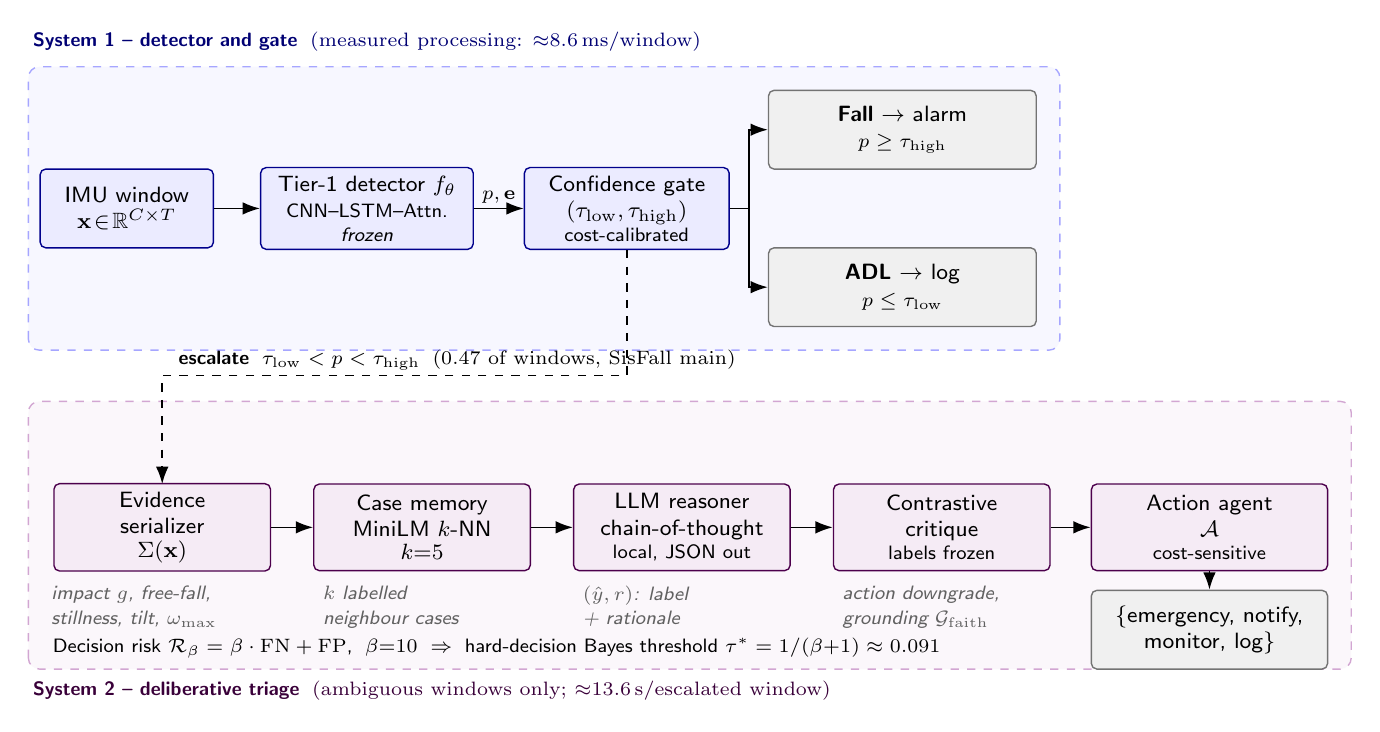
\begin{tikzpicture}[
  font=\footnotesize\sffamily,
  s1/.style={draw=blue!55!black, line width=0.5pt, rounded corners=2pt,
             fill=blue!8, align=center, inner sep=3pt,
             minimum height=1.0cm},
  s2/.style={draw=violet!60!black, line width=0.5pt, rounded corners=2pt,
             fill=violet!8, align=center, inner sep=3pt,
             minimum height=1.1cm},
  outbox/.style={draw=black!55, line width=0.5pt, rounded corners=2pt,
             fill=black!6, align=center, inner sep=3pt,
             minimum height=1.0cm},
  arr/.style={-{Latex[length=2.2mm,width=1.6mm]}, line width=0.6pt},
  darr/.style={-{Latex[length=2.2mm,width=1.6mm]}, line width=0.6pt, dashed},
  lbl/.style={font=\scriptsize\sffamily, inner sep=1.5pt},
  note/.style={font=\scriptsize\sffamily\itshape, text=black!62, inner sep=1pt}
]

% ---------- tier backdrops ----------
\draw[draw=blue!35, line width=0.5pt, dashed, rounded corners=4pt, fill=blue!3]
  (0.20,-0.30) rectangle (13.30,3.30);
\draw[draw=violet!35, line width=0.5pt, dashed, rounded corners=4pt, fill=violet!3]
  (0.20,-4.35) rectangle (17.00,-0.95);

\node[lbl, anchor=west, text=blue!45!black] at (0.20,3.62)
  {\textbf{System 1 -- detector and gate} \;\textnormal{(measured processing: $\approx$8.6\,ms/window)}};
\node[lbl, anchor=west, text=violet!45!black] at (0.20,-4.62)
  {\textbf{System 2 -- deliberative triage} \;\textnormal{(ambiguous windows only; $\approx$13.6\,s/escalated window)}};

% ---------- System 1 row ----------
\node[s1, minimum width=2.20cm] (imu)   at (1.45,1.50) {IMU window\\$\mathbf{x}\!\in\!\mathbb{R}^{C\times T}$};
\node[s1, minimum width=2.70cm] (tier1) at (4.50,1.50) {Tier-1 detector $f_\theta$\\\scriptsize CNN--LSTM--Attn.\\[-1pt]\scriptsize \emph{frozen}};
\node[s1, minimum width=2.60cm] (gate)  at (7.80,1.50) {Confidence gate\\$(\tau_{\mathrm{low}},\tau_{\mathrm{high}})$\\[-1pt]\scriptsize cost-calibrated};
\node[outbox, minimum width=3.40cm] (fall) at (11.30,2.50) {\textbf{Fall} $\rightarrow$ alarm\\\scriptsize $p\ge\tau_{\mathrm{high}}$};
\node[outbox, minimum width=3.40cm] (adl)  at (11.30,0.50) {\textbf{ADL} $\rightarrow$ log\\\scriptsize $p\le\tau_{\mathrm{low}}$};

\draw[arr] (imu) -- (tier1);
\draw[arr] (tier1) -- node[lbl, above=0pt] {$p,\mathbf{e}$} (gate);
\draw[arr] (gate.east) -- (9.35,1.50) |- (fall.west);
\draw[arr] (gate.east) -- (9.35,1.50) |- (adl.west);

% ---------- escalation link ----------
\draw[darr] (gate.south) -- (7.80,-0.62) -- (1.90,-0.62) -- (1.90,-2.00);
\node[lbl, anchor=west] at (2.05,-0.42)
  {\textbf{escalate} \;$\tau_{\mathrm{low}}<p<\tau_{\mathrm{high}}$ \;\textnormal{(0.47 of windows, SisFall main)}};

% ---------- System 2 row ----------
\node[s2, minimum width=2.75cm] (ev)   at (1.90,-2.55) {Evidence\\serializer\\[-1pt]$\Sigma(\mathbf{x})$};
\node[s2, minimum width=2.75cm] (knn)  at (5.20,-2.55) {Case memory\\MiniLM $k$-NN\\[-1pt]$k{=}5$};
\node[s2, minimum width=2.75cm] (llm)  at (8.50,-2.55) {LLM reasoner\\chain-of-thought\\[-1pt]\scriptsize local, JSON out};
\node[s2, minimum width=2.75cm] (crit) at (11.80,-2.55) {Contrastive\\critique\\[-1pt]\scriptsize labels frozen};
\node[s2, minimum width=3.00cm] (act)  at (15.20,-2.55) {Action agent\\$\mathcal{A}$\\[-1pt]\scriptsize cost-sensitive};
\node[outbox, minimum width=3.00cm] (out) at (15.20,-3.85) {\{emergency, notify,\\monitor, log\}};

\draw[arr] (ev)   -- (knn);
\draw[arr] (knn)  -- (llm);
\draw[arr] (llm)  -- (crit);
\draw[arr] (crit) -- (act);
\draw[arr] (act)  -- (out);

\node[note, anchor=north west] at (0.45,-3.25) {impact $g$, free-fall,};
\node[note, anchor=north west] at (0.45,-3.57) {stillness, tilt, $\omega_{\max}$};
\node[note, anchor=north west] at (3.90,-3.25) {$k$ labelled};
\node[note, anchor=north west] at (3.90,-3.57) {neighbour cases};
\node[note, anchor=north west] at (7.20,-3.25) {$(\hat{y},r)$: label};
\node[note, anchor=north west] at (7.20,-3.57) {+ rationale};
\node[note, anchor=north west] at (10.50,-3.25) {action downgrade,};
\node[note, anchor=north west] at (10.50,-3.57) {grounding $\mathcal{G}_{\mathrm{faith}}$};

\node[lbl, anchor=west] at (0.45,-4.08)
  {Decision risk $\mathcal{R}_\beta=\beta\cdot\mathrm{FN}+\mathrm{FP}$, \;$\beta{=}10$ \;$\Rightarrow$\; hard-decision Bayes threshold $\tau^\ast=1/(\beta{+}1)\approx0.091$};

\end{tikzpicture}
}
\caption{RCDP architecture. Every window passes the frozen Tier-1 detector and gate; measured System~1 processing latency is $8.6$\,ms on the evaluation hardware, not a wearable benchmark. Only $\tau_{\mathrm{low}}<p<\tau_{\mathrm{high}}$ escalates to evidence serialisation, retrieval and local reasoning. Critique may check rationale grounding without changing the predicted label; the Action Agent emits a simulated response. Tier-1 weights are fixed at inference. Binary FN/FP cost and graded-action evaluation are distinct.}
\label{fig:arch}
\end{figure*}

\begin{algorithm}[!t]
\caption{RCDP inference for one IMU window}
\label{alg:rcdp}
\begin{algorithmic}[1]
\REQUIRE Window $\mathbf{x}\in\mathbb{R}^{C\times T}$; frozen Tier-1 $f_\theta$; gate $(\tau_{\mathrm{low}},\tau_{\mathrm{high}})$; case memory $\mathcal{M}$; reasoner $\mathcal{L}$; critique $\mathcal{C}$; Action Agent $\mathcal{A}$; width $k$
\STATE $(\boldsymbol{\ell},\mathbf{e})\leftarrow f_\theta(\mathbf{x})$ \COMMENT{no weight update}
\STATE $p\leftarrow \mathrm{softmax}(\boldsymbol{\ell})_1$ \COMMENT{model score, \eqref{eq:pfall}}
\STATE $r\leftarrow\varnothing$ \COMMENT{no generated rationale on the edge path}
\IF{$p\le\tau_{\mathrm{low}}$}
  \STATE $\hat{y}\leftarrow\mathrm{ADL}$; \; $a\leftarrow\texttt{log}$ \COMMENT{System 1, edge}
\ELSIF{$p\ge\tau_{\mathrm{high}}$}
  \STATE $\hat{y}\leftarrow\mathrm{Fall}$; \; $a\leftarrow\texttt{emergency}$ \COMMENT{System 1, edge}
\ELSE
  \STATE \textbf{/* System 2: ambiguous band */}
  \STATE $\Sigma\leftarrow\textsc{SerializeEvidence}(\mathbf{x})$
  \STATE $N_k\leftarrow\textsc{TopK}(\mathcal{M},\Sigma,k)$ \COMMENT{cosine, \eqref{eq:cosine}}
  \STATE $(\hat{y},r)\leftarrow\mathcal{L}(\Sigma,N_k)$ \COMMENT{JSON label $+$ rationale}
  \STATE $r\leftarrow\mathcal{C}(r,\Sigma)$ \COMMENT{ground rationale; $\hat{y}$ \emph{immutable}}
  \STATE $a\leftarrow\mathcal{A}(\hat{y},r,\Sigma)$ \COMMENT{simulated graded response}
\ENDIF
\STATE \textbf{return} $(\hat{y},a,p,r)$
\end{algorithmic}
\end{algorithm}


\subsection{Tier-1 Detector}
Let $\mathbf{x}\in\mathbb{R}^{C\times T}$ be an IMU window ($C{=}6$, $T{=}90$ on SisFall). A backbone $f_\theta$ maps $\mathbf{x}$ to logits $\boldsymbol{\ell}\in\mathbb{R}^{2}$ and an embedding $\mathbf{e}$, giving
\begin{equation}
p = \hat{p}_\theta(y{=}1\mid\mathbf{x}) = \frac{e^{\ell_1}}{e^{\ell_0}+e^{\ell_1}}.
\label{eq:pfall}
\end{equation}
The primary backbone is CNN--LSTM--Attention following~\cite{bhatti2025beyond}. For context we also train a reference zoo (CNN1D, LSTM, CNN--LSTM, TCN~\cite{bai2018tcn}, ModernTCN~\cite{iglesias2023modern}, TSMixer~\cite{tsmixer2023}, PatchTST~\cite{patchtst2023}, Transformer~\cite{vaswani2017attention}) under the same protocol (Table~\ref{tab:backbone}), but every agentic table freezes \texttt{cnn\_lstm\_attn}.

\subsection{Confidence Gate}
A dual-threshold gate with calibrated $(\tau_{\mathrm{low}},\tau_{\mathrm{high}})$ routes windows:
\begin{equation}
\mathrm{route}(p)=
\begin{cases}
\mathrm{ADL}, & p \le \tau_{\mathrm{low}},\\
\mathrm{Fall}, & p \ge \tau_{\mathrm{high}},\\
\mathrm{Ambiguous}, & \text{otherwise.}
\end{cases}
\label{eq:gate}
\end{equation}
Thresholds are fit on subject-held-out calibration windows by grid search over the empirical version of~\eqref{eq:selrisk}, scoring only confident (edge) decisions under FN/FP costs plus a deferral penalty (Alg.~\ref{alg:gate}). Fig.~\ref{fig:gateband} shows the resulting decision geometry at the pooled minimum-cost point. The asymmetry is pronounced: $\tau_{\mathrm{low}}$ is pushed close to zero, so almost nothing is dismissed as ADL without deliberation, while $\tau_{\mathrm{high}}$ stays well below $1$ so that clear falls still alarm at the edge. Baseline mode \texttt{tier1\_only} removes the gate and decides with a single calibrated threshold.

\begin{figure}[!t]
\centering
\resizebox{\linewidth}{!}{% ---------------------------------------------------------------------
% Fig. 2 -- Decision geometry of the cost-calibrated dual-threshold gate.
% Pure TikZ. Thresholds shown are the pooled minimum-cost operating
% point of Table~\ref{tab:pareto} (tau_low = 0.05, tau_high = 0.60).
% Wrap with \resizebox{\linewidth}{!}{...} in main.tex.
% ---------------------------------------------------------------------
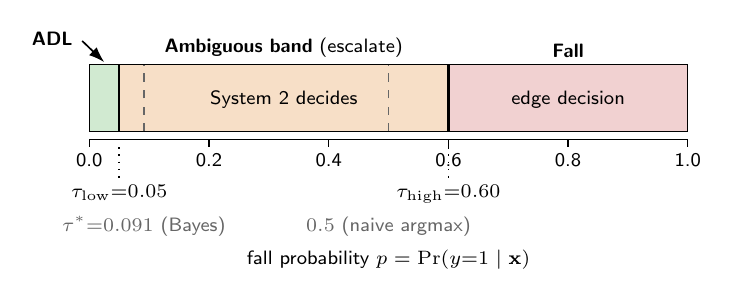
\begin{tikzpicture}[
  font=\footnotesize\sffamily,
  x=7.60cm, y=1cm,
  lbl/.style={font=\scriptsize\sffamily, inner sep=1.5pt},
  tick/.style={line width=0.5pt},
  arr/.style={-{Latex[length=2.0mm,width=1.4mm]}, line width=0.6pt}
]

% ---------- routing bands ----------
\fill[green!55!black, fill opacity=0.18] (0.00,0.00) rectangle (0.05,0.85);
\fill[orange!85!black, fill opacity=0.22] (0.05,0.00) rectangle (0.60,0.85);
\fill[red!70!black, fill opacity=0.18]    (0.60,0.00) rectangle (1.00,0.85);
\draw[line width=0.5pt] (0.00,0.00) rectangle (1.00,0.85);
\draw[line width=0.8pt] (0.05,0.00) -- (0.05,0.85);
\draw[line width=0.8pt] (0.60,0.00) -- (0.60,0.85);

% ---------- reference thresholds (inside band) ----------
\draw[dashed, line width=0.6pt, black!60] (0.091,0.00) -- (0.091,0.85);
\draw[dashed, line width=0.6pt, black!60] (0.500,0.00) -- (0.500,0.85);

% ---------- region names ----------
\node[lbl, anchor=south] at (0.325,0.88) {\textbf{Ambiguous band} (escalate)};
\node[lbl, anchor=south] at (0.800,0.88) {\textbf{Fall}};
\node[lbl, anchor=east]  at (-0.02,1.18) {\textbf{ADL}};
\draw[arr] (-0.012,1.15) -- (0.025,0.88);

\node[lbl] at (0.325,0.40) {System 2 decides};
\node[lbl] at (0.800,0.40) {edge decision};

% ---------- probability axis ----------
\draw[tick] (0.00,-0.10) -- (1.00,-0.10);
\foreach \p in {0.0,0.2,0.4,0.6,0.8,1.0}{%
  \draw[tick] (\p,-0.10) -- (\p,-0.20);
  \node[lbl, anchor=north] at (\p,-0.22) {\p};
}

% ---------- calibrated thresholds ----------
\draw[dotted, line width=0.6pt] (0.05,-0.20) -- (0.05,-0.60);
\draw[dotted, line width=0.6pt] (0.60,-0.20) -- (0.60,-0.60);
\node[lbl, anchor=north] at (0.05,-0.62) {$\tau_{\mathrm{low}}{=}0.05$};
\node[lbl, anchor=north] at (0.60,-0.62) {$\tau_{\mathrm{high}}{=}0.60$};

% ---------- reference threshold labels ----------
\node[lbl, anchor=north, text=black!60] at (0.091,-1.02) {$\tau^\ast{=}0.091$ (Bayes)};
\node[lbl, anchor=north, text=black!60] at (0.500,-1.02) {$0.5$ (naive argmax)};

\node[lbl, anchor=north] at (0.50,-1.44) {fall probability $p=\Pr(y{=}1\mid\mathbf{x})$};

\end{tikzpicture}
}
\caption{Decision geometry of the cost-calibrated gate at the pooled minimum-cost operating point (Table~\ref{tab:pareto}). Under FN-heavy cost the lower threshold collapses towards zero: the gate would rather deliberate than silently dismiss. The Bayes threshold $\tau^\ast$ of Prop.~\ref{prop:bayes} and the naive $0.5$ cut both fall \emph{inside} the ambiguous band, which is precisely why a single-threshold detector must commit where the evidence does not support committing.}
\label{fig:gateband}
\end{figure}

\begin{algorithm}[!t]
\caption{Cost-calibrated dual-threshold gate, with split-conformal audit}
\label{alg:gate}
\begin{algorithmic}[1]
\REQUIRE Subject-held-out calibration set $\{(p_i,y_i)\}_{i=1}^{n}$; costs $(\beta_{\mathrm{FN}},\beta_{\mathrm{FP}})$; deferral penalty $\lambda$; conformal level $\alpha$
\STATE \textbf{/* Routing surrogate: edge errors plus deferral penalty */}
\STATE $\mathcal{T}\leftarrow\{(t_\ell,t_h)\in \text{grid}^2 : t_\ell<t_h\}$
\FORALL{$(t_\ell,t_h)\in\mathcal{T}$}
  \STATE $E\leftarrow\{i: p_i\le t_\ell \text{ or } p_i\ge t_h\}$ \COMMENT{edge decisions}
  \STATE $J(t_\ell,t_h)\leftarrow \beta_{\mathrm{FN}}\mathrm{FN}_{E}+\beta_{\mathrm{FP}}\mathrm{FP}_{E}+\lambda\,(n-|E|)$
\ENDFOR
\STATE $(\tau_{\mathrm{low}},\tau_{\mathrm{high}})\leftarrow\arg\min_{\mathcal{T}} J$ \COMMENT{ties broken toward lower deferral}
\STATE \textbf{/* Split-conformal audit (reported, not deployed) */}
\STATE $s_i\leftarrow 1-p_i$ if $y_i{=}1$, else $s_i\leftarrow p_i$
\STATE $m\leftarrow\lceil (n{+}1)(1{-}\alpha)\rceil$
\STATE $\hat{q}\leftarrow s_{(m)}$ if $m\le n$; otherwise $\hat{q}\leftarrow+\infty$
\STATE For test $p$: $C(p)\leftarrow\{c\in\{0,1\}:\,1-\hat{p}(c)\le\hat{q}\}$
\STATE Route at the edge if $|C(p)|{=}1$; otherwise defer \COMMENT{including an empty set}
\STATE Report edge-decision FN rate and escalation rate for both gates
\STATE \textbf{return} $(\tau_{\mathrm{low}},\tau_{\mathrm{high}},\hat{q})$
\end{algorithmic}
\end{algorithm}


\subsection{Evidence Serializer}
For escalated windows we compute kinematic descriptors---free-fall duration proxy, impact magnitude, post-impact stillness, tilt change and peak angular rate---and serialise them into a natural-language evidence string $\Sigma(\mathbf{x})$ consumed by both retrieval and the reasoner. These are the primitives against which rationale grounding is later scored (Sec.~\ref{sec:clinical}).

\subsection{Retrieval Memory}
A $k$-NN memory stores MiniLM~\cite{minilm2020} embeddings of evidence text together with labels and features. On escalation we retrieve $k{=}5$ neighbours by cosine similarity as few-shot context~\cite{lewis2020rag}:
\begin{equation}
\mathrm{sim}(\mathbf{u},\mathbf{v})=\frac{\mathbf{u}^\top\mathbf{v}}{\|\mathbf{u}\|_2\|\mathbf{v}\|_2}.
\label{eq:cosine}
\end{equation}
The memory is populated from training-fold windows only, so no test subject ever appears among its own neighbours.

\subsection{LLM Reasoner}
A local reasoner (Ollama/Mistral-7B by default; heuristic and Qwen2.5-Coder-7B-Instruct backends for comparison) consumes $\Sigma(\mathbf{x})$ and retrieved neighbours and returns a JSON label and rationale~\cite{wei2022cot,mistral2023,qwen2024,ollama}. The supplied runtime tags are \texttt{mistral:latest} and \texttt{qwen2.5-coder:7b-instruct}; a mutable tag does not uniquely identify model weights. Inference runs on a local host rather than a third-party API; this is not evidence of execution on wearable hardware. Full-stack primary rows use the Mistral backend.

\subsection{Action Agent and Clinical Cost}
The Action Agent maps severity cues to simulated actions $\{\texttt{emergency},\texttt{notify},\texttt{monitor},\texttt{log}\}$. Aggregate evaluation cost follows~\eqref{eq:risk} with $\beta{=}10$, reported per $1000$ windows so that equal-budget folds are directly comparable. Sensitivity to $\beta$ is reported for $\beta\in\{5,10,20\}$ in Table~\ref{tab:betacost}.

A deliberate design restriction: the critique stage may downgrade an \emph{action} and may demand better grounding, but it may not flip a fall label to ADL. Sec.~\ref{sec:negative} shows what happens when that restriction is lifted.

\subsection{System Modes}
Ablations instantiate the cumulative ladder \texttt{tier1\_only}, \texttt{gate\_only}, \texttt{gate\_knn}, \texttt{gate\_llm} and \texttt{gate\_knn\_llm}, isolating whether the gain requires retrieval, language-model reasoning, or both.

\subsection{Deployment Timing}
\label{sec:deployment}
System~1 has millisecond processing latency on the evaluation hardware, whereas local adjudication takes seconds (Fig.~\ref{fig:timeline}). Caregiver-facing triage is the intended use, motivated by the consequences of delayed assistance~\cite{fleming2008longlie}, not pre-impact protection such as airbag deployment. No clinical deadline is validated here. Processing latency excludes window acquisition, communication and queueing; it does not establish that a serial reasoner can sustain a continuous overlapping-window stream. An embedded implementation and a measured streaming workload are needed to establish that feasibility.

\begin{figure}[!t]
\centering
\resizebox{\linewidth}{!}{% ---------------------------------------------------------------------
% Fig. 3 -- Latency budget of the two tiers on a logarithmic time axis.
% Marker values are the five-fold means of Table~\ref{tab:latency}
% (Tier-1 8.56 ms; escalated path 13.63 s).
% Pure TikZ. Wrap with \resizebox{\linewidth}{!}{...} in main.tex.
% ---------------------------------------------------------------------
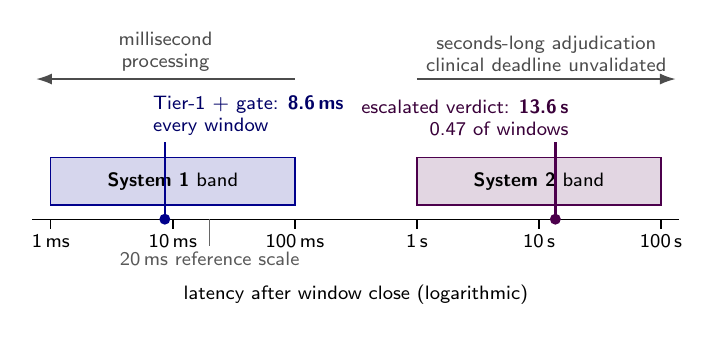
\begin{tikzpicture}[
  font=\footnotesize\sffamily,
  x=1.55cm, y=1cm,
  lbl/.style={font=\scriptsize\sffamily, inner sep=1.5pt},
  tick/.style={line width=0.5pt},
  arr/.style={-{Latex[length=2.0mm,width=1.4mm]}, line width=0.6pt}
]

% ---------- tier occupancy bands (x is log10 of time in ms) ----------
\fill[blue!55!black, fill opacity=0.16] (0.00,0.18) rectangle (2.00,0.78);
\draw[draw=blue!55!black, line width=0.5pt] (0.00,0.18) rectangle (2.00,0.78);
\node[lbl, align=center] at (1.00,0.48) {\textbf{System 1} band};

\fill[violet!60!black, fill opacity=0.16] (3.00,0.18) rectangle (5.00,0.78);
\draw[draw=violet!60!black, line width=0.5pt] (3.00,0.18) rectangle (5.00,0.78);
\node[lbl, align=center] at (4.00,0.48) {\textbf{System 2} band};

% ---------- time axis ----------
\draw[tick] (-0.15,0.00) -- (5.15,0.00);
\foreach \d/\t in {0/1\,ms, 1/10\,ms, 2/100\,ms, 3/1\,s, 4/10\,s, 5/100\,s}{%
  \draw[tick] (\d,0.00) -- (\d,-0.12);
  \node[lbl, anchor=north] at (\d,-0.14) {\t};
}

% ---------- external reference point ----------
\draw[line width=0.5pt, black!60] (1.301,0.00) -- (1.301,-0.34);
\node[lbl, anchor=north, text=black!65] at (1.301,-0.36)
  {20\,ms reference scale};

\node[lbl, anchor=north] at (2.50,-0.78) {latency after window close (logarithmic)};

% ---------- measured operating points ----------
\draw[line width=0.9pt, blue!55!black] (0.934,0.00) -- (0.934,0.98);
\node[circle, fill=blue!55!black, inner sep=1.4pt] at (0.934,0.00) {};
\node[lbl, anchor=south west, align=left, text=blue!40!black] at (0.80,1.00)
  {Tier-1 $+$ gate: \textbf{8.6\,ms}\\every window};

\draw[line width=0.9pt, violet!60!black] (4.134,0.00) -- (4.134,0.98);
\node[circle, fill=violet!60!black, inner sep=1.4pt] at (4.134,0.00) {};
\node[lbl, anchor=south east, align=right, text=violet!45!black] at (4.28,1.00)
  {escalated verdict: \textbf{13.6\,s}\\0.47 of windows};

% ---------- clinical budget annotations ----------
\draw[arr, black!70] (2.00,1.78) -- (-0.12,1.78);
\node[lbl, anchor=south, text=black!70, align=center] at (0.94,1.82)
  {millisecond\\processing};

\draw[arr, black!70] (3.00,1.78) -- (5.12,1.78);
\node[lbl, anchor=south, text=black!70, align=center] at (4.06,1.82)
  {seconds-long adjudication\\clinical deadline unvalidated};

\end{tikzpicture}
}
\caption{Processing timescales, not validated clinical deadlines. Markers are five-fold mean processing latencies from Table~\ref{tab:latency}; acquisition, queueing and caregiver response are not included.}
\label{fig:timeline}
\end{figure}

% =====================================================================
\section{Experimental Setup}
\label{sec:setup}

\subsection{Datasets and Splits}
We use six IMU channels from SisFall~\cite{sisfall2017}, which contains $38$ subjects, yielding approximately $1.55{\times}10^6$ windows at length $90$ and hop $10$. The reported protocol uses five subject-independent folds, with subject-held-out training/calibration data separate from test subjects. In the main capped slices, D18 and D19 coverage is enforced with a minimum of $80$ windows per code. This main-slice quota does not apply to the separate $300$-window stress set described below.

\paragraph{A constraint of the corpus that bounds our lead result}
In SisFall, elderly participants generally did not perform falls or D06, D13, D18 and D19 on medical advice; SE06, a 60-year-old judo practitioner, is an exception to the cohort restrictions~\cite{sisfall2017}. This limits the corpus's representation of older adults during the target stress activities. Activity codes alone do not identify the ages of the selected cases, and the supplied summaries do not provide an age-stratified stress-set analysis. We therefore make neither an elderly-specific sensitivity claim nor a prediction about the direction of age-related performance change.

Main tables use a homogeneous stratified budget of $n{=}1000$ windows per fold---necessary because escalated windows invoke a local LLM---with a fall-window prevalence of $0.433{\pm}0.004$ (Table~\ref{tab:confusion}). Archived $n{=}4000$ runs support budget-sensitivity and detailed ablations. The ambiguous stress benchmark uses $n{=}300$ per fold: $100$ D18/D19 non-fall stress activities, $100$ falls and $100$ other ADLs.

\paragraph{Follow-up controls}
The E1 and retrained detector-zoo runs use $20{,}000$ standard-protocol windows/fold; a separate CNN--LSTM--Attention v2 run uses $30{,}000$/fold. These are not the checkpoints/budgets of the main comparison. Feature adjudicators use $160$ escalated cases/fold, while the shared-ID backend comparison uses $150$/fold. Constant predictions on the latter set can be evaluated directly from its class totals without rerunning a model. Cross-set comparisons are descriptive, not paired treatment effects.

\paragraph{Run-level reconciliation}
Primary classification summaries use the supplied main-ablation confusion counts, once per mode per fold. These reproduce the original paired F1 and cost results. The separate agentic timing run has identical TP/FN counts but different FP/TN counts in three folds; only its latency and duty-cycle measurements are used as operational summaries. Extended-mode lists contain repeated folds and distinct runs, so their aggregate values are not treated as the mean of the five primary folds. This separation avoids substituting a favourable aggregate or combining metrics from different runs.

KFall~\cite{kfall2021} is the corpus emphasised in~\cite{bhatti2025beyond}. We evaluate binary Fall/ADL windows under the same cost model, gate calibration and five subject-independent folds. A Fold~0 $36$-class Tier-1 run is reported for context only (Table~\ref{tab:kfallmc}) and is explicitly not a multi-class leaderboard claim.

\subsection{Training and Agentic Protocol}
\label{sec:trainproto}
Locked YAML snapshots ship with this package under \texttt{configs/}
(\texttt{paper\_protocol.yaml}, \texttt{tier1\_sisfall.yaml},
\texttt{agentic.yaml}, \texttt{backbones.yaml}). Primary settings are:

\paragraph{Sensors and windows}
SisFall ADXL345 accelerometer + ITG3200 gyroscope ($C{=}6$ channels) at
$200$\,Hz; dense windows of length $T{=}90$ samples with hop $10$
($\approx 0.45$\,s windows, $50$\,ms stride). Binary Fall/ADL labels follow
the corpus activity codes; D18/D19 are non-fall stress activities.

\paragraph{Detector training}
Subject-independent five-fold splits. Within each training fold, $15\%$ of
subjects are held out for calibration/validation. Optimiser AdamW-family
defaults: learning rate $10^{-3}$, weight decay $10^{-4}$, batch size $256$,
label smoothing $0.05$, mixed precision, early stopping patience $10$
(Tier-1 config allows up to $80$ epochs; paper-protocol zoo caps
\texttt{max\_train}${}={}$40000). Mixup $\alpha{=}0.1$ (Tier-1 YAML uses
$0.2$) and positive class \texttt{pos\_weight} are enabled. Inputs are
normalised using training-fold statistics only. Decision thresholds for
\texttt{tier1\_only} are selected on the held-out calibration slice under the
declared mode (cost / Youden / max-F1); the primary agentic comparison uses
the cost-calibrated gate of Alg.~\ref{alg:gate}.

\paragraph{Gate calibration}
Default prior thresholds $(\tau_{\mathrm{low}},\tau_{\mathrm{high}}){=}(0.30,0.85)$
are replaced by a $20{\times}20$ grid search over
$\tau_{\mathrm{low}}{\in}[0.05,0.45]$ and
$\tau_{\mathrm{high}}{\in}[0.55,0.95]$, scoring only confident (edge)
decisions under $\mathrm{FN}{=}10$, $\mathrm{FP}{=}1$ plus a $0.5$ deferral
penalty on the deferred fraction (Alg.~\ref{alg:gate}). Calibration uses up to
\texttt{max\_cal}${}={}$2000 subject-held-out windows.

\paragraph{Evidence, retrieval and decoding}
Escalated windows are serialised by the fixed template in
\texttt{prompts/evidence\_serializer.txt}. Retrieval uses
\texttt{sentence-transformers/all-MiniLM-L6-v2}, cosine similarity, $k{=}5$,
memory built from training-fold windows only. The primary reasoner is local
Ollama with tag \texttt{mistral:latest}, temperature $0.1$, timeout $60$\,s,
up to $2$ retries, heuristic fallback on malformed JSON/timeouts. Comparison
backends: deterministic heuristic and \texttt{qwen2.5-coder:7b-instruct}.
System prompts are archived under \texttt{prompts/}. Mutable Ollama tags do
not pin weight digests; digest capture remains a release-time requirement.

\paragraph{Action policy (simulated)}
Severity thresholds: impact $\ge 5\,g$ or stillness $\ge 10$\,s $\rightarrow$
\texttt{emergency}; impact $\ge 3\,g$ or stillness $\ge 3$\,s $\rightarrow$
\texttt{notify\_caregiver}; otherwise \texttt{monitor} for falls. ADL with
elevated impact/free-fall cues maps to \texttt{monitor}, else \texttt{log}.
No live alerts are issued (\texttt{simulate: true}). Aggregate tables report
the binary FN/FP cost~\eqref{eq:risk}, not a four-action utility.

\paragraph{Seeds and budgets}
Primary seed $42$; Fold~0 multi-seed sweeps $\{42,43,44\}$. Main evaluation
\texttt{max\_test}${}={}$1000 with D18/D19 quota $80$/code; agentic latency
slice $1000$; LLM comparison $150$ escalated cases/fold; feature adjudicators
$160$/fold. Full numeric protocol is restated in Appendix~\ref{app:protocol}.

\subsection{Metrics and Statistics}
We report F1, recall (sensitivity), precision, specificity, false-positive rate, near-fall false-alarm rate on D18/D19, escalated-subset F1, escalation rate, normalised response cost~\eqref{eq:risk}, and latency. Full confusion matrices are given in Table~\ref{tab:confusion}.

We report means and sample standard deviations across five folds. Primary SisFall metrics and paired deltas are computed from supplied confusion counts before rounding. Paired fold-bootstrap intervals use $10^4$ resamples and seed $42$, with percentile intervals primary and BCa intervals as sensitivity summaries~\cite{efron1987bca}. These intervals are descriptive: five folds provide little information about uncertainty, and their training sets overlap. They are not independent clinical replications or subject-level confidence intervals. The two-sided exact Wilcoxon value is $0.0625$ for unanimous directions across five nonzero pairs, so these comparisons do not meet a $0.05$ significance threshold. We report effect sizes and directional consistency without substituting bootstrap exclusion of zero for confirmatory significance~\cite{demsar2006statistical}.

% =====================================================================
\section{Results}
\label{sec:results}

Table~\ref{tab:positioning} states the scope of comparison; Table~\ref{tab:bhattigaps} maps the open problems named in~\cite{bhatti2025beyond} to the component that addresses each.

\begin{table*}[!t]
\centering
\caption{Scope of this work relative to the base detector paper. The two studies optimise different objects: \cite{bhatti2025beyond} optimises a detector, we optimise the decision system wrapped around one. Consequently the only fair numerical comparison in our tables is \texttt{tier1\_only} versus \texttt{gate\_knn\_llm} on identical folds and checkpoints.}
\label{tab:positioning}
\begin{tabular}{@{}p{0.215\linewidth} p{0.33\linewidth} p{0.40\linewidth}@{}}
\toprule
Aspect & Bhatti \textit{et al.}~2025~\cite{bhatti2025beyond} & This work (RCDP) \\
\midrule
Object of optimisation & Detector architecture & Decision policy around a frozen detector \\
Primary task & Multi-phase fall/ADL classification & Detection $+$ deferral $+$ explanation $+$ response \\
Backbone & CNN--LSTM--Attention & \emph{Same} primary backbone (frozen) $+$ reference zoo \\
Uncertainty & Softmax confidence & Cost-calibrated dual threshold $(\tau_{\mathrm{low}},\tau_{\mathrm{high}})$, audited by split conformal \\
Explainability & Attention weights & Serialised biomechanical evidence $+$ grounded CoT rationale \\
Case memory & None & MiniLM $k$-NN retrieval over labelled evidence strings \\
Response policy & None & Cost-sensitive Action Agent under $\mathcal{R}_\beta$, $\beta{=}10$ \\
Primary corpus & KFall (multi-class, multi-phase) & SisFall binary $+$ D18/D19 stress set; KFall binary second-dataset check \\
Baseline we compare to & --- & \texttt{tier1\_only}: same checkpoint, same folds, same budget \\
\bottomrule
\end{tabular}
\end{table*}

\begin{table*}[!t]
\centering
\caption{Open problems named in the base detector paper~\cite{bhatti2025beyond}, and which component of RCDP addresses each. The final row is the honesty constraint on our claims.}
\label{tab:bhattigaps}
\begin{tabular}{@{}p{0.45\linewidth} p{0.50\linewidth}@{}}
\toprule
Limitation acknowledged in~\cite{bhatti2025beyond} & Corresponding RCDP component and evidence \\
\midrule
Softmax force-labels every window; residual sit/stand and near-fall confusion
 & Dual-threshold \textbf{confidence gate} routes the ambiguous band to System~2 (Tables~\ref{tab:ambiguoussisfall},~\ref{tab:conformalgate}) \\
Explainability limited to attention weights
 & Serialised biomechanical \textbf{evidence} $\Sigma(\mathbf{x})$ $+$ grounded chain-of-thought rationale, measured by $\mathcal{G}_{\mathrm{faith}}$ (Table~\ref{tab:grounding}) \\
No case memory or precedent reuse
 & MiniLM \textbf{$k$-NN retrieval} over labelled evidence strings; ablated in Tables~\ref{tab:ablation},~\ref{tab:knnk} \\
Detection only; no clinical response policy
 & Cost-sensitive \textbf{Action Agent} over $\{$emergency, notify, monitor, log$\}$ under $\mathcal{R}_\beta$ (Table~\ref{tab:betacost}) \\
No treatment of the false-negative/false-positive asymmetry
 & Gate and action thresholds calibrated to $\beta{=}10$; sensitivity reported for $\beta\in\{5,10,20\}$ (Table~\ref{tab:betacost}) \\
\midrule
Published result: $36$-class multi-phase F1 $\approx0.98$ at $\approx20$\,ms
 & \emph{Not contested.} We claim only that the same Tier-1 backbone, frozen, attains better recall and lower clinical cost under uncertainty when wrapped in RCDP (Tables~\ref{tab:perfold},~\ref{tab:kfallperfold}) \\
\bottomrule
\end{tabular}
\end{table*}


\subsection{Ambiguous Stress Benchmark (Lead Result)}
\label{sec:ambiguous}
The dedicated stress set tests discrimination between falls and challenging non-fall activities (Table~\ref{tab:ambiguoussisfall}). Tier-1 mean F1 is $0.713$ while \texttt{gate\_knn\_llm} reaches $0.896$ ($\Delta$F1 $=+0.183$, $\Delta$Recall $=+0.208$, cost per window $0.903{\rightarrow}0.148$, approximately $84\%$ lower). The improvement holds on all five folds. Escalation is high ($0.59$) on this deliberately enriched set, with one third of windows drawn from D18/D19; it is not a free-living duty-cycle estimate.

\begin{table*}[!t]
\centering
\caption{SisFall stress benchmark: $300$ windows/fold, comprising $100$ D18/D19 non-fall stress activities, $100$ falls and $100$ other ADLs. D19 is not a clinically adjudicated near-fall. Cost/win is $(10\mathrm{FN}+\mathrm{FP})/n$; Esc. is the escalation rate. Mean recall improves by $0.208$ and classification cost falls by approximately $84\%$. This enriched set is not a free-living duty-cycle estimate; age-stratified results are unavailable (Sec.~\ref{sec:setup}). F1 deltas use the displayed rounded metrics.}
\label{tab:ambiguoussisfall}
\begin{tabular}{c r ccc ccc cc}
\toprule
Fold & $n$ & \multicolumn{3}{c}{\texttt{tier1\_only}} & \multicolumn{3}{c}{\texttt{gate\_knn\_llm}} & $\Delta$F1 & Esc. \\
\cmidrule(lr){3-5}\cmidrule(lr){6-8}
 & & F1 & Rec. & Cost/win & F1 & Rec. & Cost/win & & rate \\
\midrule
0 & 300 & 0.696 & 0.790 & 0.86 & 0.868 & 0.990 & 0.13 & $+0.172$ & 0.59 \\
1 & 300 & 0.738 & 0.790 & 0.82 & 0.894 & 0.930 & 0.28 & $+0.156$ & 0.52 \\
2 & 300 & 0.682 & 0.750 & 0.98 & 0.892 & 0.990 & 0.11 & $+0.210$ & 0.63 \\
3 & 300 & 0.714 & 0.760 & 0.92 & 0.902 & 0.970 & 0.16 & $+0.188$ & 0.61 \\
4 & 300 & 0.735 & 0.750 & 0.93 & 0.922 & 1.000 & 0.06 & $+0.187$ & 0.62 \\
\midrule
Mean & 300 & 0.713 & 0.768 & 0.90 & \textbf{0.896} & \textbf{0.976} & \textbf{0.15} & \textbf{+0.183} & 0.59 \\
\bottomrule
\end{tabular}
\end{table*}


\subsection{Main Comparison against Tier-1}
On the main $n{=}1000$ protocol (Table~\ref{tab:perfold}) the stack improves F1 on every fold, by $+0.114$ to $+0.164$. Five-fold means (Table~\ref{tab:meanstd}) move F1 from $0.759$ to $0.887$, recall from $0.759$ to $0.977$, and cost per $1000$ windows from $1151$ to $200$---an $83\%$ reduction. Table~\ref{tab:stats} reports bootstrap CIs that exclude zero on all three metrics with $5/5$ fold sign consistency. Fig.~\ref{fig:costf1} shows the paired per-fold pattern.

Recall improves alongside mean precision: the main-ablation counts yield precision $0.760{\pm}0.032\rightarrow0.813{\pm}0.036$ and specificity $0.815{\pm}0.035\rightarrow0.828{\pm}0.039$ (Tables~\ref{tab:confusion}--\ref{tab:meanstd}). Mean false negatives fall from $104.6$ to $10.2$ per $1000$ windows. Specificity is averaged from exact per-fold count ratios rather than rounded displayed rates. The separate timing-run summaries ($0.813{\pm}0.038$ precision, $0.827{\pm}0.040$ specificity) are not substituted into this paired comparison. The specificity change is descriptive, not a separate significance claim.

\begin{table}[!t]
\centering
\caption{Author-supplied main-ablation confusion counts on SisFall ($n{=}1000$/fold), with metrics recomputed before rounding. These supplied counts confirm the earlier integer reconstruction, including $437$ falls in folds~1 and~3. They yield mean costs $1150.8$ and $199.8$. Counts are aggregate records, not independent verification of prediction files or case identity. The separate timing run differs by $+1$, $-1$ and $+2$ false positives in stack folds~1, 3 and~4 and is not mixed into this table.}
\label{tab:confusion}
\begin{tabular}{c rrrr ccc}
\toprule
Fold & TP & FP & FN & TN & Prec. & Spec. & FPR \\
\midrule
\multicolumn{8}{l}{\textit{\texttt{tier1\_only}}} \\
0 & 335 & 102 & 94  & 469 & 0.767 & 0.821 & 0.179 \\
1 & 327 & 123 & 110 & 440 & 0.727 & 0.782 & 0.218 \\
2 & 339 & 126 & 94  & 441 & 0.729 & 0.778 & 0.222 \\
3 & 320 & 78  & 117 & 485 & 0.804 & 0.861 & 0.139 \\
4 & 322 & 95  & 108 & 475 & 0.772 & 0.833 & 0.167 \\
\cmidrule(lr){1-8}
Mean & 328.6 & 104.8 & 104.6 & 462.0 & 0.760 & 0.815 & 0.185 \\
\midrule
\multicolumn{8}{l}{\textit{\texttt{gate\_knn\_llm}}} \\
0 & 423 & 96  & 6  & 475 & 0.815 & 0.832 & 0.168 \\
1 & 398 & 100 & 39 & 463 & 0.799 & 0.822 & 0.178 \\
2 & 432 & 124 & 1  & 443 & 0.777 & 0.781 & 0.219 \\
3 & 435 & 63  & 2  & 500 & 0.873 & 0.888 & 0.112 \\
4 & 427 & 106 & 3  & 464 & 0.801 & 0.814 & 0.186 \\
\cmidrule(lr){1-8}
Mean & 423.0 & 97.8 & \textbf{10.2} & 469.0 & \textbf{0.813} & \textbf{0.828} & \textbf{0.172} \\
\bottomrule
\end{tabular}
\end{table}


\begin{figure}[!t]
\centering
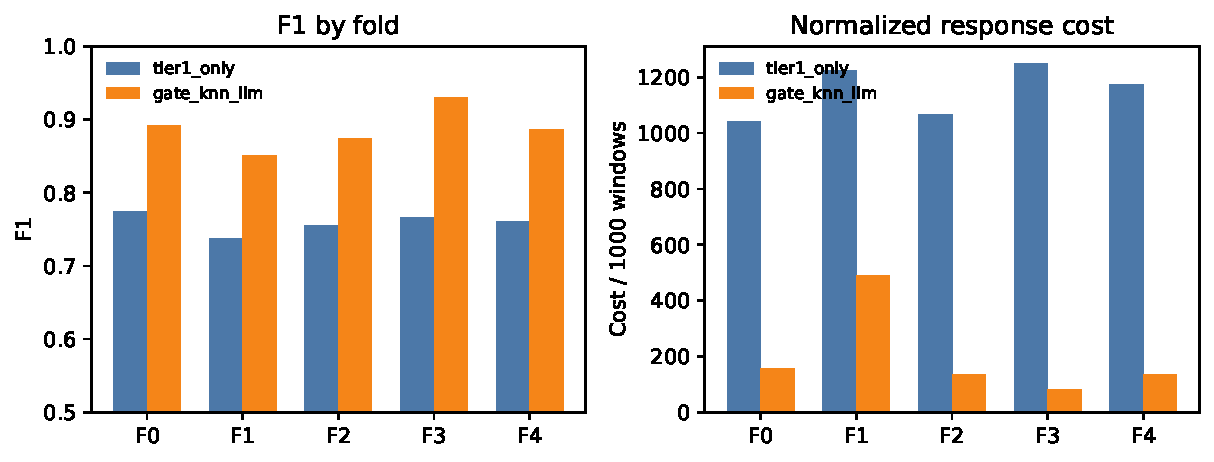
\includegraphics[width=\linewidth]{figures/cost_f1_per_fold.pdf}
\caption{Per-fold F1 and normalised response cost for \texttt{tier1\_only} versus \texttt{gate\_knn\_llm} under the homogeneous $n{=}1000$ protocol. Both metrics move in the intended direction on every fold.}
\label{fig:costf1}
\end{figure}

\begin{table*}[!t]
\centering
\caption{Per-fold comparison of the frozen Tier-1 detector (\texttt{tier1\_only}) against the full agentic stack (\texttt{gate\_knn\_llm}) under the homogeneous SisFall protocol: $n{=}1000$ stratified windows per fold with forced D18/D19 near-fall coverage, subject-independent folds, identical checkpoints. Cost is $10\cdot\mathrm{FN}{+}\mathrm{FP}$ normalised per $1000$ windows. The stack improves F1, recall and cost on \emph{every} fold; aggregate statistics and CIs are in Tables~\ref{tab:meanstd}--\ref{tab:stats}.}
\label{tab:perfold}
\begin{tabular}{c r ccc ccc cc}
\toprule
Fold & $n$ & \multicolumn{3}{c}{\texttt{tier1\_only}} & \multicolumn{3}{c}{\texttt{gate\_knn\_llm}} & $\Delta$F1 & $\Delta$Cost \\
\cmidrule(lr){3-5}\cmidrule(lr){6-8}
 & & F1 & Rec. & Cost/1k & F1 & Rec. & Cost/1k & & \\
\midrule
0 & 1000 & 0.774 & 0.781 & 1042 & 0.892 & 0.986 & 156 & $+0.119$ & $-886$  \\
1 & 1000 & 0.737 & 0.748 & 1223 & 0.851 & 0.911 & 490 & $+0.114$ & $-733$  \\
2 & 1000 & 0.755 & 0.783 & 1066 & 0.874 & 0.998 & 134 & $+0.119$ & $-932$  \\
3 & 1000 & 0.766 & 0.732 & 1248 & 0.930 & 0.995 & 83  & $+0.164$ & $-1165$ \\
4 & 1000 & 0.760 & 0.749 & 1175 & 0.887 & 0.993 & 136 & $+0.126$ & $-1039$ \\
\midrule
Mean & 1000 & 0.759 & 0.759 & 1151 & \textbf{0.887} & \textbf{0.977} & \textbf{200} & \textbf{+0.128} & $-951$ \\
\bottomrule
\end{tabular}
\end{table*}

\begin{table}[!t]
\centering
\caption{Main-ablation evaluation, five-fold mean$\pm$sample std on SisFall ($n{=}1000$/fold, prevalence $0.433{\pm}0.004$). All metrics are computed from the supplied counts in Table~\ref{tab:confusion} before rounding. No operating-point metrics from the separate timing run are substituted. Paired intervals are descriptive fold-bootstrap summaries (Table~\ref{tab:stats}).}
\label{tab:meanstd}
\begin{tabular}{lccccc}
\toprule
Mode & F1 & Recall & Prec. & Spec. & Cost/1000 \\
\midrule
\texttt{tier1\_only}
 & 0.759 & 0.759 & 0.760 & 0.815 & 1151 \\
 & {\scriptsize$\pm$0.014} & {\scriptsize$\pm$0.022} & {\scriptsize$\pm$0.032} & {\scriptsize$\pm$0.035} & {\scriptsize$\pm$93} \\
\addlinespace
\textbf{\texttt{gate\_knn\_llm}}
 & \textbf{0.887} & \textbf{0.977} & \textbf{0.813} & \textbf{0.828} & \textbf{200} \\
 & {\scriptsize$\pm$0.029} & {\scriptsize$\pm$0.037} & {\scriptsize$\pm$0.036} & {\scriptsize$\pm$0.039} & {\scriptsize$\pm$164} \\
\midrule
\multicolumn{6}{l}{\textit{Paired $\Delta$ (stack $-$ Tier-1), percentile bootstrap 95\% CI}} \\
\midrule
F1        & \multicolumn{5}{l}{$+0.128$ \quad $[0.117,\ 0.147]$ \quad 5/5 folds} \\
Recall    & \multicolumn{5}{l}{$+0.218$ \quad $[0.187,\ 0.248]$ \quad 5/5 folds} \\
Cost/1000 & \multicolumn{5}{l}{$-951$ \quad\; $[-1079,\ -825]$ \quad 5/5 folds} \\
\bottomrule
\end{tabular}
\end{table}

\begin{table}[!t]
\centering
\caption{Descriptive paired statistics across five SisFall test folds. Deltas use metrics computed from main-ablation counts before rounding. Fold-bootstrap percentile intervals use $10^4$ resamples, seed $42$; BCa sensitivity intervals are F1 $[0.117,0.154]$, recall $[0.181,0.244]$ and cost $[-1084,-834]$. With only five folds and overlapping training sets, these are not population-level significance guarantees. The two-sided exact Wilcoxon value $0.0625$ does not meet a $0.05$ significance threshold. \emph{Sign} counts folds with the favourable direction.}
\label{tab:stats}
\begin{tabular}{lcccc}
\toprule
Metric & Mean $\Delta$ & Percentile 95\% CI & Sign & Wilcoxon $p$ \\
\midrule
F1         & $+0.128$ & $[0.117,\ 0.147]$ & 5/5 & 0.0625 \\
Recall     & $+0.218$ & $[0.187,\ 0.248]$ & 5/5 & 0.0625 \\
Cost/1000  & $-951$   & $[-1079,\ -825]$  & 5/5 & 0.0625 \\
\bottomrule
\end{tabular}
\end{table}

% Regenerate with: python recompute_ci.py
% Source: main_ablation in results_text/reported_counts.csv, before rounding.


\subsection{Is It Just Threshold Moving?}
\label{sec:thresholdcontrol}
An economical explanation of a recall gain under FN-heavy cost is a lower threshold. We therefore test a single cut at $\tau^\ast{=}0.091$ without deferral, motivated by Prop.~\ref{prop:bayes}. Since posterior calibration is not established, this is a specified operating-point control, not proof that every single-threshold alternative is inferior.

Table~\ref{tab:partitionfallback} evaluates it. Recall is $0.988{\pm}0.008$, marginally above the stack's $0.977$. Plugging aggregate F1 $0.639$, recall $0.988$ and prevalence $0.433$ into the binary metric identities gives approximately $478$ false positives per $1000$ windows, specificity $0.16$ and classification cost $530$. These are approximate aggregate estimates, not measured mean fold metrics, because the transformations are nonlinear. The estimated cost is lower than Tier-1's $1151$ but about $2.6$ times the stack's $200$.

The stack therefore improves on this particular recall-oriented threshold control in both F1 and estimated classification cost. This does not establish superiority to every calibrated detector or demonstrate reduced caregiver alarm fatigue, which requires prospective evaluation.

\begin{table}[!t]
\centering
\caption{\textbf{Fixed-threshold control.} Threshold $\tau^\ast{=}1/(\beta{+}1){=}0.091$ for $\beta{=}10$, without deferral (SisFall, $n{=}1000$/fold). Bayes optimality requires calibrated posteriors; better empirically tuned thresholds are not ruled out. Values marked $^\dagger$ are approximate plug-in estimates from rounded aggregate F1, recall and main-run prevalence, not fold-wise measurements. All stack classification metrics use main-ablation counts, as in Table~\ref{tab:meanstd}; escalation is from the separate timing run.}
\label{tab:partitionfallback}
\begin{tabular}{lcc}
\toprule
Metric & $\tau^\ast$ fallback & \texttt{gate\_knn\_llm} \\
\midrule
F1              & 0.639 $\pm$ 0.006 & \textbf{0.887 $\pm$ 0.029} \\
Recall          & \textbf{0.988 $\pm$ 0.008} & 0.977 $\pm$ 0.037 \\
Precision       & 0.47$^\dagger$ & \textbf{0.813 $\pm$ 0.036} \\
Specificity     & 0.16$^\dagger$ & \textbf{0.828 $\pm$ 0.039} \\
Cost/1000       & $\approx$530$^\dagger$ & \textbf{200 $\pm$ 164} \\
Escalation rate & 0.00 & 0.47 \\
\bottomrule
\end{tabular}
\end{table}


\subsection{Ablations}
On Fold~0 at the archived $n{=}4000$ budget (Table~\ref{tab:ablation}, Fig.~\ref{fig:ablation}) and in the main five-fold evaluation (Table~\ref{tab:ablationmean}), \texttt{gate\_only} reproduces \texttt{tier1\_only}. This is a classification-only null control, not evidence that deferral is free. Main-run \texttt{gate\_knn} is mildly harmful (F1 $0.759{\rightarrow}0.753$; cost $1151{\rightarrow}1286$), while \texttt{gate\_llm} raises recall to $0.895$ but reduces precision. In the archived Fold~0 run, near-fall false-alarm rate rises from $0.219$ to $0.625$ without retrieval; the joint configuration reaches F1 $0.907$, recall $0.993$ and escalated-subset F1 $0.952$, with cost $4596{\rightarrow}516$. These results support complementarity in this implementation. Aggregating the supplied main counts reproduces stack F1 $0.887{\pm}0.029$ and cost $199.8$; the extended-mode aggregate $0.877{\pm}0.071$ is not the mean/std of these five folds and is not used as their estimate.

\begin{figure}[!t]
\centering
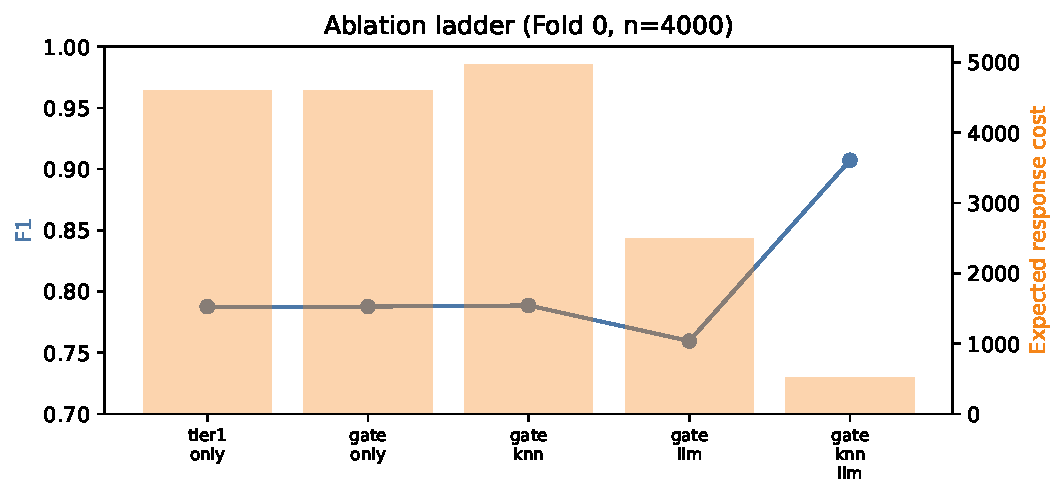
\includegraphics[width=\linewidth]{figures/ablation_ladder.pdf}
\caption{Ablation ladder on Fold~0 ($n{=}4000$ archive): F1 (left axis) and expected response cost (right axis).}
\label{fig:ablation}
\end{figure}

\begin{table}[!t]
\centering
\caption{Cumulative ablation ladder on SisFall Fold~0 under the full archived budget ($n{=}4000$). \emph{Cost} is the absolute clinical cost $10\cdot\mathrm{FN}{+}\mathrm{FP}$ and \emph{Cost/1k} the same quantity normalised per $1000$ windows for comparison with Table~\ref{tab:perfold}. \texttt{gate\_only} reproduces \texttt{tier1\_only} exactly because, with no System~2 attached, deferred windows fall back to Tier-1 \texttt{argmax}; only its escalated-subset F1 differs. \texttt{gate\_llm} buys recall at the price of a near-tripled near-fall false-alarm rate. Retrieval and language-model reasoning are complementary: neither alone reaches the full stack.}
\label{tab:ablation}
\begin{tabular}{lccrrcc}
\toprule
Mode & F1 & Recall & Cost & Cost/1k & Near-fall FAR & Esc.\ F1 \\
\midrule
\texttt{tier1\_only} & 0.788 & 0.787 & 4596 & 1149 & 0.219 & --- \\
\texttt{gate\_only}  & 0.788 & 0.787 & 4596 & 1149 & 0.219 & 0.175 \\
\texttt{gate\_knn}   & 0.789 & 0.764 & 4972 & 1243 & 0.188 & 0.026 \\
\texttt{gate\_llm}   & 0.760 & 0.924 & 2491 & 623  & 0.625 & 0.445 \\
\textbf{\texttt{gate\_knn\_llm}} & \textbf{0.907} & \textbf{0.993} & \textbf{516} & \textbf{129} & 0.212 & \textbf{0.952} \\
\bottomrule
\end{tabular}
\end{table}

\begin{table}[!t]
\centering
\caption{Main-ablation evaluation, five-fold mean$\pm$sample std recomputed from supplied per-fold confusion counts ($n{=}1000$/fold). Each mode contributes once per fold. \texttt{gate\_only} and \texttt{tier1\_only} have identical counts; cost excludes deferral overhead. These rows reproduce the original main comparison. Extended-mode exports contain repeated folds and distinct runs and are not pooled into this estimate.}
\label{tab:ablationmean}
\begin{tabular}{lccc}
\toprule
Mode & F1 & Recall & Cost/1000 \\
\midrule
\texttt{tier1\_only} & 0.759$\pm$0.014 & 0.759$\pm$0.022 & 1151$\pm$93 \\
\texttt{gate\_only}  & 0.759$\pm$0.014 & 0.759$\pm$0.022 & 1151$\pm$93 \\
\texttt{gate\_knn}   & 0.753$\pm$0.012 & 0.723$\pm$0.032 & 1286$\pm$133 \\
\texttt{gate\_llm}   & 0.702$\pm$0.021 & 0.895$\pm$0.027 & 740$\pm$105 \\
\texttt{gate\_knn\_llm} & 0.887$\pm$0.029 & 0.977$\pm$0.037 & 200$\pm$164 \\
\bottomrule
\end{tabular}
\end{table}


\subsection{Reasoner Backends on the Ambiguous Band}
Table~\ref{tab:llm} and Fig.~\ref{fig:llm} compare backends on shared escalated case IDs ($150$/fold). The heuristic achieves F1 $0.034{\pm}0.044$ and recall $0.018{\pm}0.023$, consistent with ADL-biased predictions. Mistral-7B reaches F1 $0.972{\pm}0.010$ and Qwen2.5-Coder-7B-Instruct $0.823{\pm}0.029$. Both have zero observed false negatives on these cases, but their specificities differ: $0.891$ versus $0.195$. Their count-derived costs are $37.3$ and $280.0$ per $1000$ escalated cases (Table~\ref{tab:adjudicator}). Zero observed misses on a selected finite subset is not a population safety guarantee.

\begin{figure}[!t]
\centering
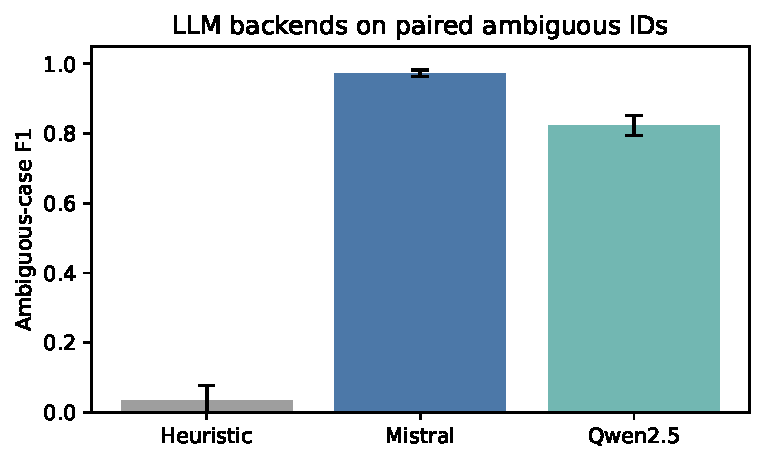
\includegraphics[width=0.9\linewidth]{figures/llm_backends.pdf}
\caption{Mean$\pm$std ambiguous-case F1 across five folds for the heuristic, Mistral-7B and Qwen2.5 backends on shared case IDs.}
\label{fig:llm}
\end{figure}

\begin{table}[!t]
\centering
\caption{Paired backend F1 on SisFall, using the reported same $150$ escalated case IDs/fold and supplied evidence/neighbours. Qwen denotes \texttt{qwen2.5-coder:7b-instruct}. Count-derived costs and an always-fall control on these same class totals appear in Table~\ref{tab:adjudicator}. The feature-classifier set is separate, so this is not a matched comparison against GBM.}
\label{tab:llm}
\begin{tabular}{cccc}
\toprule
Fold & Heuristic F1 & Mistral-7B F1 & Qwen2.5 F1 \\
\midrule
0 & 0.042 & 0.959 & 0.807 \\
1 & 0.105 & 0.977 & 0.874 \\
2 & 0.000 & 0.975 & 0.819 \\
3 & 0.021 & 0.984 & 0.802 \\
4 & 0.000 & 0.966 & 0.813 \\
\midrule
Mean$\pm$std & 0.034$\pm$0.044 & \textbf{0.972$\pm$0.010} & 0.823$\pm$0.029 \\
\bottomrule
\end{tabular}
\end{table}


\subsection{Is a Language Model Necessary?}
\label{sec:adjudicatorcontrol}
Table~\ref{tab:adjudicator} separates two case sets. On the feature-based evaluation ($160$/fold), always-fall achieves F1 $0.814$ and cost $311.3$ per $1000$ cases, compared with GBM F1 $0.780$ and cost $1366.3$. The constant rule has lower cost on all five folds; it does not have higher F1 on every fold. Logistic regression, random and ADL-biased heuristic controls further show why the heuristic alone is insufficient. These are the tested feature classifiers, not evidence that all cost-tuned classifiers would fail.

For prevalence $q$, always-fall has recall $1$, specificity $0$, F1 $2q/(1+q)$ and cost $1000(1-q)$. Applying these identities to the \emph{LLM set's own} class totals yields F1 $0.790{\pm}0.028$ and cost $346.7{\pm}39.7$. Both LLMs improve on this matched constant control; Qwen is therefore not equivalent to always-fall. Mistral reduces its mean classification cost by approximately $89\%$ while retaining zero observed false negatives. The feature and LLM case sets still differ, so no matched GBM--Mistral effect is estimated. The results show discrimination beyond a constant prediction, not that an LLM is uniquely necessary or more efficient than a cost-tuned classifier with identical evidence and retrieval context.

\begin{table*}[!t]
\centering
\caption{Adjudicator controls on two distinct SisFall escalated-case evaluations. Entries are five-fold mean$\pm$sample std, recomputed from supplied confusion counts. Cost is $(10\mathrm{FN}+\mathrm{FP})/n\times1000$ within the escalated subset, excluding compute cost. Panel A has $160$ cases/fold; panel B has $150$ shared cases/fold. Panel B's always-fall row is derived exactly from its class totals, not borrowed from panel A. Comparisons are valid within panels; the table does not provide a matched GBM--Mistral comparison. Training-majority predictions coincide with always-fall in panel A.}
\label{tab:adjudicator}
\begin{tabular}{lcccc}
\toprule
Method & F1 & Recall & Specificity & Cost/1000 escalated \\
\midrule
\multicolumn{5}{l}{\textit{A: Feature-based adjudication ($n=160$/fold)}} \\
Always fall & 0.814$\pm$0.044 & 1.000$\pm$0.000 & 0.000$\pm$0.000 & 311.3$\pm$63.3 \\
Always ADL & 0.000$\pm$0.000 & 0.000$\pm$0.000 & 1.000$\pm$0.000 & 6887.5$\pm$633.4 \\
Training majority & 0.814$\pm$0.044 & 1.000$\pm$0.000 & 0.000$\pm$0.000 & 311.3$\pm$63.3 \\
Random & 0.605$\pm$0.057 & 0.536$\pm$0.041 & 0.488$\pm$0.088 & 3348.8$\pm$330.6 \\
Heuristic & 0.039$\pm$0.011 & 0.020$\pm$0.006 & 0.981$\pm$0.022 & 6755.0$\pm$654.5 \\
Logistic regression & 0.664$\pm$0.102 & 0.599$\pm$0.129 & 0.571$\pm$0.106 & 2856.3$\pm$755.8 \\
Gradient boosting & 0.780$\pm$0.046 & 0.831$\pm$0.040 & 0.338$\pm$0.118 & 1366.3$\pm$297.4 \\
\midrule
\multicolumn{5}{l}{\textit{B: Shared-ID backend comparison ($n=150$/fold)}} \\
Always fall (derived) & 0.790$\pm$0.028 & 1.000$\pm$0.000 & 0.000$\pm$0.000 & 346.7$\pm$39.7 \\
Heuristic (LLM set) & 0.034$\pm$0.044 & 0.018$\pm$0.023 & 0.992$\pm$0.010 & 6416.0$\pm$285.4 \\
Mistral-7B & 0.972$\pm$0.010 & 1.000$\pm$0.000 & 0.891$\pm$0.036 & 37.3$\pm$13.0 \\
Qwen2.5-Coder-7B & 0.823$\pm$0.029 & 1.000$\pm$0.000 & 0.195$\pm$0.045 & 280.0$\pm$41.6 \\
\bottomrule
\end{tabular}
\end{table*}

\subsection{Clinical Cost Framing and Rationale Grounding}
\label{sec:clinical}
Table~\ref{tab:betacost} reports sensitivity to the cost ratio. The stack's advantage is monotone in $\beta$: the more a deployment penalises missed falls, the larger the absolute saving ($-479$, $-951$, $-1895$ per $1000$ windows at $\beta=5,10,20$). This matters because $\beta$ is a site-specific clinical parameter, not a constant of nature.

A language model asked to justify a safety decision can produce fluent severity language unsupported by telemetry~\cite{huang2025hallucination}. We therefore measure kinematic faithfulness $\mathcal{G}_{\mathrm{faith}}$: the fraction of rationales citing at least one primitive actually present in $\Sigma(\mathbf{x})$ (Table~\ref{tab:grounding}). Contrastive critique raises mean $\mathcal{G}_{\mathrm{faith}}$ from $0.436$ to $0.843$ and cuts graded action cost by $45\%$ ($589{\rightarrow}324$). $\mathcal{G}_{\mathrm{faith}}$ is a faithfulness proxy, not a correctness measure: a rationale can cite the right primitive and still reach the wrong conclusion. We report it because an ungrounded rationale is unusable for clinical audit even when the label happens to be right.

\begin{table}[!t]
\centering
\caption{Sensitivity to the clinical cost ratio $\beta=c_{\mathrm{FN}}/c_{\mathrm{FP}}$ (SisFall, five-fold mean cost per $1000$ windows, $\mathcal{R}_\beta=\beta\cdot\mathrm{FN}+\mathrm{FP}$). The advantage of the stack is monotone in $\beta$: the more a deployment penalises missed falls relative to nuisance alarms, the larger the absolute saving. $\tau^\ast=1/(\beta{+}1)$ is the corresponding hard-decision Bayes threshold~\eqref{eq:tau_star}. The $\beta{=}10$ row is the paper's primary setting.}
\label{tab:betacost}
\begin{tabular}{ccl rr}
\toprule
$\beta$ & $\tau^\ast$ & Mode & Cost/1000 & $\Delta$ vs.\ Tier-1 \\
\midrule
5  & 0.167 & \texttt{tier1\_only} & 628 & --- \\
5  & 0.167 & \textbf{\texttt{gate\_knn\_llm}} & \textbf{149} & $-479$ \\
\addlinespace
10 & 0.091 & \texttt{tier1\_only} & 1151 & --- \\
10 & 0.091 & \textbf{\texttt{gate\_knn\_llm}} & \textbf{200} & $-951$ \\
\addlinespace
20 & 0.048 & \texttt{tier1\_only} & 2197 & --- \\
20 & 0.048 & \textbf{\texttt{gate\_knn\_llm}} & \textbf{302} & $-1895$ \\
\bottomrule
\end{tabular}
\end{table}

\begin{table}[!t]
\centering
\caption{Rationale grounding. $\mathcal{G}_{\mathrm{faith}}$ is the fraction of LLM rationales that cite at least one primitive actually present in the evidence string $\Sigma(\mathbf{x})$ (impact magnitude, free-fall proxy, post-impact stillness, tilt change, peak angular rate); it is a faithfulness proxy, not a correctness measure. \emph{Graded cost} is the cost of the Action Agent's four-level output rather than the binary label. Contrastive critique with frozen labels nearly doubles grounding ($0.436{\rightarrow}0.843$) and cuts graded action cost by $45\%$, in contrast to the label-flipping critic of Table~\ref{tab:negative}.}
\label{tab:grounding}
\begin{tabular}{ccccc}
\toprule
\multirow{2}{*}{Fold} & \multicolumn{2}{c}{$\mathcal{G}_{\mathrm{faith}}$} & \multicolumn{2}{c}{Graded action cost} \\
\cmidrule(lr){2-3}\cmidrule(lr){4-5}
 & base & $+$critique & base & $+$critique \\
\midrule
0 & 0.430 & 0.851 & 544 & 268 \\
1 & 0.340 & 0.749 & 901 & 599 \\
2 & 0.471 & 0.871 & 535 & 261 \\
3 & 0.482 & 0.874 & 428 & 216 \\
4 & 0.459 & 0.868 & 537 & 274 \\
\midrule
Mean & 0.436 & \textbf{0.843} & 589 & \textbf{324} \\
\bottomrule
\end{tabular}
\end{table}


\subsection{Negative Study: Label-Flip Actor--Critic}
\label{sec:negative}
Permitting a Critic to flip fall$\rightarrow$ADL labels is unsafe under FN-heavy cost, and we report the magnitude rather than omitting the experiment. Table~\ref{tab:negative} shows mean false negatives rising from $12.4$ to $116.2$ per $1000$ windows---a factor of $9.4$---with mean recall collapsing from $0.971$ to $0.732$ and mean F1 from $0.891$ to $0.761$. The effect is consistent on all five folds; on Fold~3, false negatives rise from $3$ to $122$. The mechanism is intuitive: a critic optimising for plausibility finds it easy to argue that an ambiguous window was "probably just sitting down", and every such argument costs $\beta$.

We therefore (i) freeze fall/ADL labels in the primary stack, (ii) restrict critique to action downgrades and rationale grounding, and (iii) prefer contrastive hard negatives to unconstrained vetoes. Not every additional agent helps, and in a safety-critical loop the default should be that a new agent may refine a response but may not overturn a positive detection.

\begin{table}[!t]
\centering
\caption{\textbf{Negative result.} Naive label-flip Actor--Critic (\texttt{gate\_knn\_llm\_actor\_critic}) versus the primary stack on SisFall ($n{=}1000$/fold). Permitting the Critic to veto fall predictions inflates false negatives by an order of magnitude, which is the exact failure mode an FN-heavy cost penalises. Contrastive action critique with \emph{frozen} labels is the safe alternative (Table~\ref{tab:grounding}). Both columns come from one paired actor--critic run; its \texttt{gate\_knn\_llm} column therefore differs by ${\le}0.022$ F1 from Table~\ref{tab:perfold}, which reflects non-deterministic local-LLM decoding rather than a protocol change.}
\label{tab:negative}
\begin{tabular}{c ccc ccc c}
\toprule
Fold & \multicolumn{3}{c}{\texttt{gate\_knn\_llm}} & \multicolumn{3}{c}{$+$Actor--Critic (harmful)} & $\Delta$FN \\
\cmidrule(lr){2-4}\cmidrule(lr){5-7}
 & F1 & Rec. & FN & F1 & Rec. & FN & \\
\midrule
0 & 0.893 & 0.986 & 6  & 0.768 & 0.755 & 105 & $+99$  \\
1 & 0.851 & 0.911 & 39 & 0.744 & 0.714 & 125 & $+86$  \\
2 & 0.896 & 0.986 & 6  & 0.757 & 0.725 & 119 & $+113$ \\
3 & 0.917 & 0.993 & 3  & 0.766 & 0.721 & 122 & $+119$ \\
4 & 0.898 & 0.981 & 8  & 0.769 & 0.744 & 110 & $+102$ \\
\midrule
Mean & 0.891 & 0.971 & 12.4 & 0.761 & 0.732 & 116.2 & $+103.8$ \\
\bottomrule
\end{tabular}
\end{table}


\subsection{Escalation Duty Cycle}
Table~\ref{tab:escalation} reports escalation rates per protocol: $0.47{\pm}0.08$ on SisFall main, $0.59{\pm}0.04$ on the stress set, and $0.011$ on binary KFall. The SisFall figures are high and materially constrain deployability. Stratification and near-fall enrichment prevent interpreting them as free-living estimates or guaranteed upper bounds; distribution shift could change duty cycle in either direction. KFall illustrates a lower duty cycle under a different, easier binary evaluation, not a deployment guarantee. Holding conditional risks fixed, $\pi$ scales the benefit of escalation without changing its sign.

\begin{table}[!t]
\centering
\caption{System~2 duty cycle by evaluation protocol. The $1000$-window SisFall rate comes from the separate timing run, not the primary classification counts. SisFall protocols are stratified and D18/D19 enriched: these rates constrain feasibility but are neither free-living estimates nor guaranteed upper bounds. Distribution shift can change escalation in either direction. Binary KFall invokes deliberation on roughly one window in ninety under its own protocol.}
\label{tab:escalation}
\begin{tabular}{lcc}
\toprule
Protocol & $n$/fold & Escalation rate \\
\midrule
SisFall timing (5-fold mean)    & 1000 & 0.47 $\pm$ 0.08 \\
SisFall ambiguous stress        & 300  & 0.59 $\pm$ 0.04 \\
KFall external (5-fold mean)    & 1000 & 0.011 \\
\bottomrule
\end{tabular}
\end{table}


\subsection{Backbone Context}
Table~\ref{tab:backbone} replaces single-fold architecture context with the E1 and retrained five-fold detector runs. ModernTCN has the highest mean F1 in each ($0.743$ and $0.760$ from displayed fold values); CNN--LSTM--Attention has $0.717$ and $0.739$. A separate v2 run at $30{,}000$ windows/fold reaches $0.751{\pm}0.039$ (Table~\ref{tab:g1primary}). Its cost-oriented and maximum-F1-labelled settings give approximately $0.664$ and $0.743$ when recomputed from the supplied rounded folds. These labels describe threshold-selection settings, not test-set optimality guarantees.

The separate standard/enriched summaries show small changes for most backbones, but PatchTST is an exception ($0.541{\rightarrow}0.672$). These evaluations differ in prevalence and operating-point context and cannot isolate an enrichment effect. Per-backbone D18/D19-specific results are unavailable. Thus the tested configurations have modest dense-window performance, but neither an architecture-independent ceiling nor a field-wide near-fall collapse is established. The main paired $0.759{\rightarrow}0.887$ comparison remains tied to its frozen checkpoints; complete matched wrapper evaluation across the zoo is not available.

\begin{table}[!t]
\centering
\caption{Five-fold detector-only SisFall context at the reported Youden operating points, $20{,}000$ standard-protocol windows/fold (prevalence $0.329$--$0.345$). E1 and retrained zoo are distinct checkpoint runs. Mean$\pm$sample std are recomputed from the supplied three-decimal fold F1 values; last-digit differences from separately supplied aggregate summaries can result from rounding. Neither run is the frozen main comparison or the separate $30{,}000$-window v2 evaluation. Scores describe tested implementations and training settings, not a universal architecture ranking.}
\label{tab:backbone}
\begin{tabular}{lcc}
\toprule
Model & E1 F1 & Retrained F1 \\
\midrule
CNN1D & 0.701$\pm$0.031 & 0.734$\pm$0.026 \\
LSTM & 0.693$\pm$0.016 & 0.711$\pm$0.026 \\
CNN--LSTM & 0.696$\pm$0.010 & 0.724$\pm$0.036 \\
CNN--LSTM--Attention & 0.717$\pm$0.022 & 0.739$\pm$0.030 \\
TCN & 0.702$\pm$0.029 & 0.747$\pm$0.034 \\
ModernTCN & 0.743$\pm$0.015 & 0.760$\pm$0.030 \\
TSMixer & 0.671$\pm$0.022 & 0.686$\pm$0.018 \\
PatchTST & 0.541$\pm$0.009 & 0.566$\pm$0.014 \\
Transformer & 0.690$\pm$0.013 & 0.703$\pm$0.017 \\
\bottomrule
\end{tabular}
\end{table}

\begin{table*}[!t]
\centering
\caption{Separate CNN--LSTM--Attention v2 detector evaluation on $30{,}000$ standard-protocol windows/fold, without the wrapper. Thresholds and metrics are supplied fold summaries at the Youden operating point; aggregate cells are recomputed from the displayed rounded metrics. Fall prevalence ranges from $0.328$ to $0.347$. These checkpoints and budgets differ from the main $n=1000$ paired comparison and the $n=20{,}000$ zoo; their scores are not substituted for the main Tier-1 baseline.}
\label{tab:g1primary}
\begin{tabular}{ccccccc}
\toprule
Fold & F1 & Recall & Specificity & Precision & Accuracy & Threshold \\
\midrule
0 & 0.760 & 0.853 & 0.809 & 0.685 & 0.823 & 0.347 \\
1 & 0.683 & 0.763 & 0.756 & 0.617 & 0.758 & 0.401 \\
2 & 0.768 & 0.775 & 0.879 & 0.761 & 0.845 & 0.563 \\
3 & 0.783 & 0.850 & 0.838 & 0.726 & 0.842 & 0.374 \\
4 & 0.761 & 0.797 & 0.842 & 0.728 & 0.826 & 0.500 \\
\midrule
Mean$\pm$std & 0.751$\pm$0.039 & 0.808$\pm$0.042 & 0.825$\pm$0.046 & 0.703$\pm$0.055 & 0.819$\pm$0.035 & --- \\
\bottomrule
\end{tabular}
\end{table*}

\subsection{Latency and Budget Sensitivity}
Table~\ref{tab:latency} and Fig.~\ref{fig:latency} report the separate timing run: Tier-1 processing is $8.56$\,ms and the escalated path averages $13.64$\,s, dominated by local decoding. Mean per-window processing is $6.37$\,s at duty cycle $0.468$. This run has stack F1 $0.887{\pm}0.030$ and mean cost $200.2$, close to but distinct from the main-ablation values; its operational measurements are not an exact replay of the primary classification run. Fig.~\ref{fig:budget} reports archived $n{=}1000$/$4000$ comparisons. Similar directions across these budgets support a sensitivity check, not a guarantee against selection bias or a streaming-throughput claim.

\begin{figure}[!t]
\centering
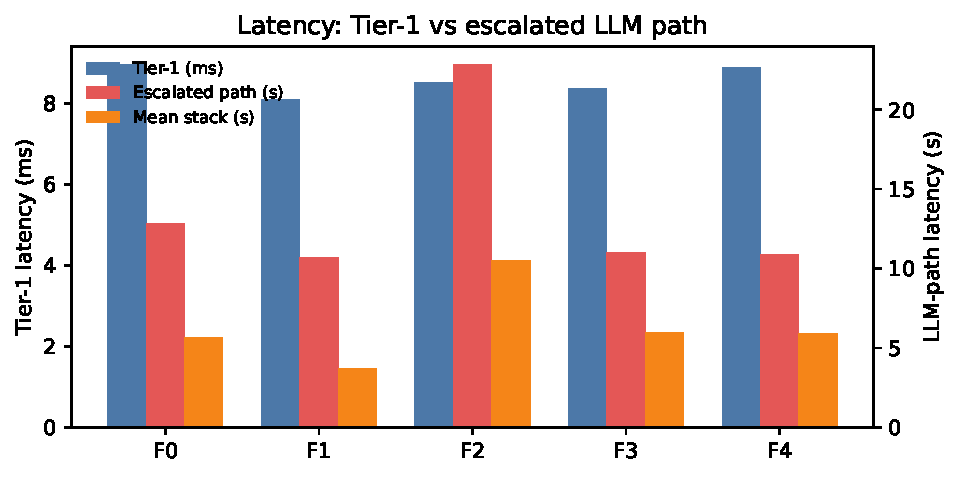
\includegraphics[width=\linewidth]{figures/latency_bars.pdf}
\caption{Latency by fold: Tier-1 (ms, left axis) versus escalated LLM path and mean stack latency (seconds, right axis).}
\label{fig:latency}
\end{figure}

\begin{figure}[!t]
\centering
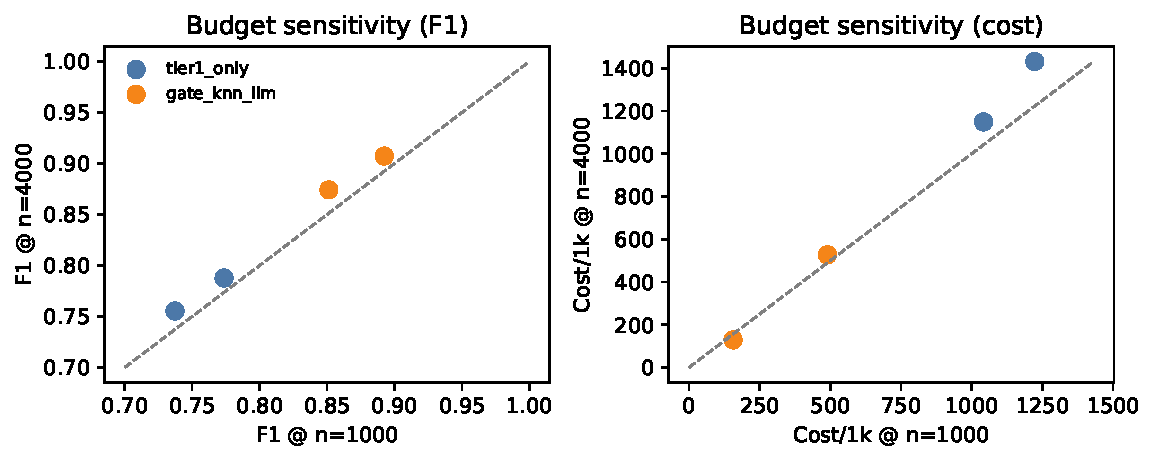
\includegraphics[width=\linewidth]{figures/budget_sensitivity.pdf}
\caption{Budget sensitivity: metrics at $n{=}1000$ versus $n{=}4000$ for Tier-1 and the full stack on archived folds.}
\label{fig:budget}
\end{figure}

\begin{table}[!t]
\centering
\caption{Processing latency from the separate Ollama/Mistral agentic timing run (SisFall, $n{=}1000$/fold; GPU evaluation, not wearable hardware). Tier-1 is evaluated for every window; the escalated path is dominated by local LLM decoding. Mean stack is the measured per-window average. Fold~2 has the slowest escalated path ($22.85$\,s), not the highest duty cycle (its rate is $0.460$, versus $0.546$ on Fold~4). Window acquisition, queueing and clinical response time are not established by these measurements.}
\label{tab:latency}
\begin{tabular}{crrr}
\toprule
Fold & Tier-1 (ms) & Escalated (s) & Mean stack (s) \\
\midrule
0 & 8.96 & 12.81 & 5.68 \\
1 & 8.09 & 10.66 & 3.73 \\
2 & 8.52 & 22.85 & 10.52 \\
3 & 8.36 & 11.00 & 5.99 \\
4 & 8.89 & 10.86 & 5.93 \\
\midrule
Mean & 8.56 & 13.64 & 6.37 \\
\bottomrule
\end{tabular}
\end{table}


\subsection{External Validation on KFall}
\label{sec:kfall}
Tables~\ref{tab:kfallperfold}--\ref{tab:kfallmean} evaluate the decision layer on a second dataset using a binary Fall/ADL protocol. Tier-1 F1 is $0.987{\pm}0.005$ against $0.990{\pm}0.004$ for the stack ($\Delta$F1 $=+0.003$), with cost per $1000$ falling from $50$ to $26$. This is a second-dataset consistency check, not evidence of zero-shot transfer of a SisFall-trained model or formal non-inferiority: Fold~1 regresses and the descriptive F1 interval touches zero. The largest difference in displayed fold values is $+0.009$ on Fold~4. Fold~0 ablations and backends appear in Tables~\ref{tab:kfallablation}--\ref{tab:kfallllm}; the $36$-class context run is Table~\ref{tab:kfallmc}.

\begin{table*}[!t]
\centering
\caption{Second-dataset evaluation on KFall, frozen Tier-1 versus full stack under the binary Fall/ADL protocol ($n{=}1000$/fold). This is not evidence of zero-shot transfer of SisFall-trained weights or formal non-inferiority. Fold~1 regresses; Fold~4 has the largest displayed F1 gain. Deltas below are computed from the displayed rounded values.}
\label{tab:kfallperfold}
\begin{tabular}{c r ccc ccc cc}
\toprule
Fold & $n$ & \multicolumn{3}{c}{\texttt{tier1\_only}} & \multicolumn{3}{c}{\texttt{gate\_knn\_llm}} & $\Delta$F1 & $\Delta$Cost \\
\cmidrule(lr){3-5}\cmidrule(lr){6-8}
 & & F1 & Rec. & Cost/1k & F1 & Rec. & Cost/1k & & \\
\midrule
0 & 1000 & 0.992 & 0.998 & 17  & 0.993 & 1.000 & 7  & $+0.001$ & $-10$ \\
1 & 1000 & 0.987 & 0.996 & 31  & 0.986 & 0.996 & 32 & $-0.001$ & $+1$  \\
2 & 1000 & 0.987 & 0.994 & 40  & 0.989 & 0.996 & 29 & $+0.002$ & $-11$ \\
3 & 1000 & 0.992 & 0.990 & 53  & 0.995 & 0.996 & 23 & $+0.003$ & $-30$ \\
4 & 1000 & 0.980 & 0.979 & 109 & 0.989 & 0.994 & 38 & $+0.009$ & $-71$ \\
\midrule
Mean & 1000 & 0.987 & 0.991 & 50 & \textbf{0.990} & \textbf{0.996} & \textbf{26} & $+0.003$ & $-24.2$ \\
\bottomrule
\end{tabular}
\end{table*}

\begin{table}[!t]
\centering
\caption{KFall external validation, five-fold mean$\pm$std (binary Fall/ADL, $n{=}1000$ windows/fold). Deltas are \texttt{gate\_knn\_llm}$-$\texttt{tier1\_only} over the same checkpoints and folds; intervals are percentile bootstrap ($10^{4}$ resamples, seed $42$). Tier-1 is already near ceiling, so this is a \emph{stability} check, not an improvement claim: the F1 interval touches zero and one fold regresses. We omit Wilcoxon $p$-values here because one recall delta is exactly zero, leaving four effective pairs---too few for the test to be informative.}
\label{tab:kfallmean}
\begin{tabular}{lccc}
\toprule
Mode & F1 & Recall & Cost/1000 \\
\midrule
\texttt{tier1\_only}   & 0.987$\pm$0.005 & 0.991$\pm$0.007 & 50$\pm$35 \\
\textbf{\texttt{gate\_knn\_llm}} & \textbf{0.990$\pm$0.004} & \textbf{0.996$\pm$0.002} & \textbf{26$\pm$12} \\
\midrule
\multicolumn{4}{l}{\textit{Paired $\Delta$ (stack $-$ Tier-1)}} \\
\midrule
Metric & Mean $\Delta$ & Percentile 95\% CI & Sign \\
\midrule
F1        & $+0.003$  & $[0.000,\ 0.006]$  & 4/5 \\
Recall    & $+0.005$  & $[0.001,\ 0.010]$  & 4/5 \\
Cost/1000 & $-24.2$   & $[-48.4,\ -5.8]$   & 4/5 \\
\bottomrule
\end{tabular}
\end{table}

\begin{table}[!t]
\centering
\caption{KFall Fold~0 cumulative ablation ($n{=}1000$, binary). Cost is already per $1000$ windows. As on SisFall, \texttt{gate\_only} reproduces \texttt{tier1\_only} exactly and the joint retrieval$+$reasoner configuration is the only one that improves both recall and cost. Absolute headroom is small because Tier-1 is near ceiling on this corpus.}
\label{tab:kfallablation}
\begin{tabular}{lccrc}
\toprule
Mode & F1 & Recall & Cost/1k & Esc.\ F1 \\
\midrule
\texttt{tier1\_only} & 0.992 & 0.998 & 17 & --- \\
\texttt{gate\_only}  & 0.992 & 0.998 & 17 & 0.750 \\
\texttt{gate\_knn}   & 0.991 & 0.994 & 36 & 0.400 \\
\texttt{gate\_llm}   & 0.976 & 0.998 & 33 & 0.250 \\
\textbf{\texttt{gate\_knn\_llm}} & \textbf{0.993} & \textbf{1.000} & \textbf{7} & \textbf{0.889} \\
\bottomrule
\end{tabular}
\end{table}

\begin{table}[!t]
\centering
\caption{KFall paired reasoner comparison on shared escalated case IDs. Because KFall escalation is rare ($\approx1.1\%$ of windows), each fold contributes only a handful of cases; the spread across folds is correspondingly wide and we read the ordering, not the levels.}
\label{tab:kfallllm}
\begin{tabular}{cccc}
\toprule
Fold & Heuristic F1 & Mistral-7B F1 & Qwen2.5 F1 \\
\midrule
0 & 0.167 & 0.880 & 0.500 \\
1 & 0.000 & 1.000 & 0.364 \\
2 & 0.000 & 1.000 & 0.600 \\
3 & 0.000 & 0.571 & 0.250 \\
4 & 0.273 & 0.974 & 0.809 \\
\midrule
Mean$\pm$std & 0.088$\pm$0.126 & \textbf{0.885$\pm$0.182} & 0.504$\pm$0.216 \\
\bottomrule
\end{tabular}
\end{table}

\begin{table}[!t]
\centering
\caption{Context only: our Tier-1 backbone trained as a $36$-class transition-phase classifier on KFall Fold~0. This row exists to state plainly what our training budget and preprocessing achieve in the multi-class setting, and it is \textbf{not} a comparison against the published multi-phase result---the protocols, window definitions, label granularity and training budgets differ. All of the paper's claims are made in the binary Fall/ADL setting of Table~\ref{tab:kfallperfold}.}
\label{tab:kfallmc}
\begin{tabular}{lccc}
\toprule
Setting & Acc. & Macro-F1 & Weighted-F1 \\
\midrule
Our Tier-1 ($36$-class, Fold~0) & 0.585 & 0.541 & 0.583 \\
Bhatti \textit{et al.}~\cite{bhatti2025beyond} (published, \emph{different protocol}) & --- & $\approx$0.98 & --- \\
\bottomrule
\end{tabular}
\end{table}


\subsection{Split-Conformal Gating, Robustness and Duty-Cycle Trade-offs}
\label{sec:conformal}
The binary split-conformal rule uses nonconformity $s=1-\hat{p}(y)$ and finite-sample quantile $\hat{q}$~\cite{vovk2005algorithmic,angelopoulos2023gentle}: singleton prediction sets route at the edge; non-singleton sets, including empty sets, defer in the stated rule. Table~\ref{tab:conformalgate} audits routing at $\alpha{=}0.05$. On folds~0--3, edge false-negative rates are $0.010$--$0.030$ with escalation $0.58$--$0.83$, compared with $0.38$--$0.47$ for the cost gate. Fold~4 has a lower quantile ($0.630$), escalation $0.17$ and edge FN rate $0.087$. Standard split conformal controls marginal prediction-set miscoverage under exchangeability, not the false-negative rate conditional on being a fall and being resolved at the edge. Thus comparing these edge FN rates with $\alpha$ neither verifies nor refutes nominal coverage. Subject shift and overlapping windows also warrant caution about exchangeability, but this audit does not identify the cause of the fold variation or establish a conditional safety guarantee. The production gate remains cost-calibrated.

Table~\ref{tab:pareto} summarises duty-cycle Pareto points and notes that the nominal cost minimiser is dominated by a configuration with the same cost and $23$ percentage points less escalation. Table~\ref{tab:robustness} shows graceful degradation under sensor perturbation: clean F1 $0.768{\pm}0.017$ against $0.754{\pm}0.023$ at $\pm15^\circ$ frame rotation, with resampling to $50$/$100$\,Hz costing $0.002$. Table~\ref{tab:knnk} sweeps retrieval width $k\in\{1,5,10\}$ under the heuristic backend and is flat by construction, since that backend ignores neighbour labels; it is a null control, and a sweep under a language-model backend remains open.

\begin{table}[!t]
\centering
\caption{Split-conformal routing audit at $\alpha{=}0.05$. \emph{Esc.} is the escalation rate and \emph{Edge FN} the false-negative rate restricted to windows resolved at the edge. Edge FN is not marginal prediction-set miscoverage and is not guaranteed to be below $\alpha$. The audit partition is a subject-held-out calibration/test split drawn separately from the main protocol, so escalation rates are not directly comparable with Table~\ref{tab:escalation}. Both gates report identical F1 because escalated windows revert to Tier-1 \texttt{argmax}, not System~2; the audit measures routing, not stack accuracy.}
\label{tab:conformalgate}
\begin{tabular}{c ccc ccc}
\toprule
 & \multicolumn{4}{c}{Split conformal} & \multicolumn{2}{c}{Cost gate} \\
\cmidrule(lr){2-5}\cmidrule(lr){6-7}
Fold & $\hat{q}$ & Esc. & Edge FN & F1 & Esc. & F1 \\
\midrule
0 & 0.830 & 0.58 & 0.017 & 0.774 & 0.38 & 0.774 \\
1 & 0.926 & 0.83 & 0.030 & 0.737 & 0.47 & 0.737 \\
2 & 0.904 & 0.70 & 0.017 & 0.764 & 0.40 & 0.764 \\
3 & 0.856 & 0.61 & 0.010 & 0.787 & 0.38 & 0.787 \\
4 & 0.630 & 0.17 & \textbf{0.087} & 0.778 & 0.22 & 0.778 \\
\midrule
Mean & 0.829 & 0.58 & 0.032 & 0.768 & 0.37 & 0.768 \\
\bottomrule
\end{tabular}
\end{table}

\begin{table}[!t]
\centering
\caption{Archived pooled routing diagnostic without System~2. The entries labelled min-cost and Q25 tie at reported cost $1015$, while Q25 has $23$ percentage points less deferral. Under these displayed objectives, min-cost is dominated; the source selection rule and the treatment of deferred-case errors must be distinguished from the production routing surrogate. These pooled points do not justify choosing deployment thresholds without held-out calibration and adjudicator evaluation.}
\label{tab:pareto}
\begin{tabular}{lcccr}
\toprule
Operating point & $\tau_{\mathrm{low}}$ & $\tau_{\mathrm{high}}$ & Esc.\ rate & Cost \\
\midrule
Min cost            & 0.05 & 0.60 & 0.57 & 1015 \\
\textbf{Q25 esc.\ (dominant)} & \textbf{0.30} & \textbf{0.70} & \textbf{0.34} & \textbf{1015} \\
Q50 esc.            & 0.40 & 0.95 & 0.48 & 1042 \\
Q75 esc.            & 0.30 & 0.95 & 0.61 & 1223 \\
\bottomrule
\end{tabular}
\end{table}

\begin{table}[!t]
\centering
\caption{Sensor-perturbation robustness of Tier-1 routing under the cost gate (SisFall, five-fold mean F1). Rotations apply a random rigid rotation of the sensor frame with the stated bound, emulating garment or mounting drift; resampling emulates a different device sampling rate. Degradation is graceful---the worst case, $\pm15^\circ$, loses $0.014$ F1---so the ambiguous band is not an artefact of one exact sensor placement.}
\label{tab:robustness}
\begin{tabular}{lcc}
\toprule
Condition & Mean F1 & $\Delta$ vs.\ clean \\
\midrule
clean             & 0.768 $\pm$ 0.017 & --- \\
resample 100\,Hz  & 0.766 $\pm$ 0.016 & $-0.002$ \\
resample 50\,Hz   & 0.766 $\pm$ 0.015 & $-0.002$ \\
rotate $\pm10^\circ$ & 0.763 $\pm$ 0.020 & $-0.005$ \\
rotate $\pm15^\circ$ & 0.754 $\pm$ 0.023 & $-0.014$ \\
\bottomrule
\end{tabular}
\end{table}

\begin{table}[!t]
\centering
\caption{Retrieval-width ablation, $k\in\{1,5,10\}$ (SisFall Fold~0, main protocol). The reasoner here is the \emph{heuristic} backend, which consumes the evidence string but ignores neighbour labels; the result is consequently flat by construction and should be read as a null control confirming that retrieval width cannot rescue an incompetent reasoner---not as evidence that $k$ is irrelevant to the Mistral stack. A retrieval-width sweep under a language-model backend is left to future work (Sec.~\ref{sec:limitations}).}
\label{tab:knnk}
\begin{tabular}{cccc}
\toprule
$k$ & F1 & Recall & Escalation \\
\midrule
1  & 0.384 & 0.240 & 0.38 \\
5  & 0.384 & 0.240 & 0.38 \\
10 & 0.384 & 0.240 & 0.38 \\
\bottomrule
\end{tabular}
\end{table}


% =====================================================================
\section{Discussion}
\label{sec:discussion}

\subsection{What Changes Relative to Detection-Only Work}
The main comparison is \texttt{tier1\_only} versus \texttt{gate\_knn\_llm} on the reported shared SisFall folds and checkpoints (Table~\ref{tab:positioning}). SisFall supplies the explicit D18/D19 activity codes used for the stress evaluation, not clinical near-fall adjudication. KFall multi-class multi-phase analysis remains the setting of~\cite{bhatti2025beyond}; our binary KFall evaluation is a second-dataset check, not a competing multi-phase result.

Published SisFall results must also be interpreted under their own metrics and protocols. For example, Waheed \textit{et al.}~\cite{waheed2021ntfds} report $97.21\%$ accuracy for NT-FDS; this is not directly comparable with fall-class F1 on our subject-independent dense-window evaluation. A common dataset name does not align windowing, label assignment, subject splits, prevalence or operating points. Without a matched reproduction, the follow-up does not show that published detectors collapse on near-falls, nor identify the cause of the numerical gap.

\subsection{Where the Gains Come From}
The main comparison shows higher recall on every fold and lower FN-weighted classification cost under the assumed cost ratio. The joint retrieval--reasoning configuration also achieves escalated-subset F1 $0.952$ on the archived Fold~0 run. These observations support selective adjudication in the evaluated system, but F1 alone cannot establish $r_1-r_2>\lambda$ for an unmeasured deployment cost. The reported ablations favour the joint configuration; the unmatched feature-baseline follow-up does not isolate the necessity of language-model reasoning. Near-fall false-alarm improvements are modest and are not presented as a differentiator.

\subsection{Statistics, Seeds and Reproducibility}
Table~\ref{tab:stats} reports paired deltas with percentile CIs as primary, BCa sensitivity intervals, and $5/5$ directional consistency. Multi-seed Fold~0 sweeps (Table~\ref{tab:seeds}) give stack F1 $0.905{\pm}0.005$ across seeds $\{42,43,44\}$, a spread an order of magnitude below the effect being claimed. Because seeds redraw the stratified slice as well as training randomness, absolute values differ slightly from the locked Fold~0 row; the quantity of interest is the spread.

\begin{table}[!t]
\centering
\caption{Multi-seed robustness on SisFall Fold~0 ($n{=}1000$, Ollama/Mistral backend). Seeds redraw the stratified test slice as well as training randomness, so absolute values differ from the Fold~0 row of Table~\ref{tab:perfold} (which uses the locked seed-42 slice); the quantity of interest is the across-seed spread, not the level.}
\label{tab:seeds}
\begin{tabular}{ccccc}
\toprule
Seed & Tier-1 F1 & Stack F1 & Stack Rec. & Cost/1000 \\
\midrule
42 & 0.747 & 0.909 & 0.998 & 95 \\
43 & 0.740 & 0.907 & 0.995 & 105 \\
44 & 0.746 & 0.899 & 1.000 & 96 \\
\midrule
Mean$\pm$std & 0.745$\pm$0.004 & \textbf{0.905$\pm$0.005} & 0.998$\pm$0.003 & 99$\pm$6 \\
\bottomrule
\end{tabular}
\end{table}


\subsection{Limitations}
\label{sec:limitations}
We state these in the order a reviewer should weigh them.

\emph{Duty cycle.} Escalation is substantial on SisFall ($0.47$ main, $0.59$ stress) and the escalated path costs seconds on a local 7B model. We make no sub-$5\%$ duty-cycle claim, and on a battery-powered wearable this cost is real; we did not profile energy or embedded deployment, so the on-device feasibility of System~2 is unestablished. A distilled or quantised on-device reasoner is the obvious next step.

\emph{Effect size on KFall.} $\Delta$F1 is $+0.003$ and one fold regresses. We report it as a stability check and would not defend it as an improvement.

\emph{Statistical power.} Five folds and overlapping training sets limit inferential claims. Fold-bootstrap intervals are descriptive; the exact paired test does not reach $p<0.05$. Overlapping windows also mean that window counts should not be interpreted as independent clinical events. Subject-level uncertainty and event-level false alarms per unit time remain unmeasured.

\emph{Simulated actions.} The Action Agent's outputs are simulated. We have no live clinical trial, no caregiver-in-the-loop study, and therefore no evidence about alarm fatigue or real dispatch outcomes---the very quantities $\beta$ is meant to encode.

\emph{Conformal scope.} Edge false-negative rates vary across folds and are not the marginal miscoverage quantity controlled by standard split conformal. The audit therefore supplies no conditional edge-FN guarantee. Exchangeability under subject shift and overlapping windows requires separate assessment (Sec.~\ref{sec:conformal}).

\emph{Open ablations.} Retrieval width is swept only under the heuristic backend; the memory is not updated online; and the reasoner comparison covers two open-weight models at one size. A matched always-fall control is now available for the LLM set, but feature classifiers use different cases. Identical-case comparisons with cost-tuned feature classifiers and matched evidence remain necessary to isolate language-model value over those alternatives.

\emph{Backbone generality.} The follow-up's best observed F1 near $0.76$ is protocol- and training-dependent, not a universal ceiling. Standard-versus-enriched results do not establish near-fall degradation for every architecture. The main paired gains concern one frozen backbone; a wrapper evaluation across all reference backbones and a harmonised audit of retraining balance, checkpoints and threshold selection remain outstanding.

\emph{Age and clinical generalisability.} SisFall's elderly activity restrictions limit the target activities available for evaluation. The supplied stress-set summaries contain no age-stratified results. Neither older-adult near-fall performance nor the direction of age-related distribution shift is established here.

\emph{Record provenance.} Supplied per-fold confusion counts resolve the earlier integer-reconstruction ambiguity and permit count-based aggregation. They do not independently establish case identity, subject disjointness or absence of leakage. Raw predictions, split manifests, preprocessing configurations and immutable model identifiers remain necessary for full reproduction. Distinct classification, timing and extended-mode runs are kept separate.

\emph{Reasoner reliability.} Non-deterministic decoding means the escalated path is not bitwise reproducible, which is why the actor--critic study in Table~\ref{tab:negative} is reported as its own paired run.

Free-living unlabelled streams, distilled on-device reasoners and prospective eldercare validation remain future work.

% =====================================================================
\section{Conclusion}
\label{sec:concl}

We evaluated a confidence-gated decision layer around a fixed CNN--LSTM--Attention detector. Under the main SisFall protocol, retrieval-augmented adjudication improves F1, recall and FN-weighted classification cost on every fold and outperforms the tested fixed-threshold control. Count-based reconciliation preserves these paired gains while separating classification and timing runs. On shared escalated cases, Mistral also improves on a matched always-fall control, demonstrating discrimination beyond prevalence alone. The results do not establish architecture-independent gains or LLM necessity over matched feature classifiers. Substantial adjudication latency, limited older-adult evidence and descriptive five-fold uncertainty constrain deployment claims. The contribution is a protocol-specific decision-layer evaluation; clinical utility requires prospective study.

% =====================================================================
\section*{Ethical and Data-Use Statement}
This study uses previously published public datasets, SisFall~\cite{sisfall2017} and KFall~\cite{kfall2021}, with collection ethics documented by their original authors. No new participant data were collected for this retrospective analysis. Local language-model inference avoids a third-party inference API. Action outputs are simulated: no alerts or clinical interventions were evaluated. The intended role is caregiver-facing decision support, not autonomous emergency response. The cost ratio encodes an assumption, not a clinically validated utility. Before submission the authors must confirm secondary-data compliance with their institution and the dataset licenses; this manuscript does not claim a new IRB approval number.

\section*{Author Declarations (to complete before submission)}
\label{sec:authordecls}
\textbf{Authors / affiliations / ORCID / corresponding author:} placeholders above; complete in \texttt{AUTHOR\_DECLARATIONS.md}.
\textbf{Contributions:} to be supplied (CRediT).
\textbf{Funding:} to be supplied (grant IDs) or state ``None''.
\textbf{Conflicts of interest:} to be supplied or state ``The authors declare no competing interests.''
\textbf{Acknowledgments:} optional.
These fields are intentionally blank rather than fabricated.

\section*{Data and Code Availability}
The Overleaf package includes: (i)~table/figure/algorithm sources; (ii)~verification scripts; (iii)~transcribed per-fold records in \texttt{results\_text/} (\texttt{reported\_counts.csv}, \texttt{backbone\_f1.csv}, \texttt{g1\_v2.csv}); (iv)~locked YAML under \texttt{configs/}; (v)~system prompts and the evidence serializer template under \texttt{prompts/}. Together these support numerical reconstruction and configuration inspection of the reported protocol. Window-level prediction exports and subject-split manifests for the primary runs live in the companion experiment tree (documented in the parent repository's \texttt{RESULT\_EXPORTS\_INDEX.md}: \texttt{results/fold\{0--4\}/}, \texttt{results/standard\_protocol*}, \texttt{results/adjudicator\_compare/}). SisFall and KFall remain available from their original authors. A complete public code+weight release is not claimed in this package; digests for mutable Ollama tags should be recorded at camera-ready time.

% =====================================================================
\appendices

\section{Reproducibility Notes}
\label{app:repro}
The supplied records distinguish main-ablation classification, a separate
agentic timing run, feature adjudication and shared-ID LLM adjudication.
Five-fold means use one observation per fold rather than pooling repeated
extended-mode exports. Count-derived metrics are calculated before rounding;
detector-zoo summaries use the available rounded fold metrics.

The following checks use the included records and require no LaTeX installation:
\begin{verbatim}
python check_manuscript.py   # inputs, labels, cite keys, table arity
python check_numbers.py      # available Mean rows vs. displayed folds
python check_reported_results.py # counts and selected aggregates
python recompute_ci.py       # descriptive paired fold intervals
\end{verbatim}
The historical \texttt{recover\_confusion.py} script is retained for the earlier
integer reconstruction; supplied counts now provide the primary arithmetic
source. These checks do not establish case identity, leakage-free splits or
clinical validity. Intervals in Tables~\ref{tab:stats} and~\ref{tab:kfallmean}
use SisFall counts and displayed KFall fold values, respectively.

\section{Homogeneous Protocol Details}
\label{app:protocol}
This appendix restates the locked settings shipped under \texttt{configs/}
and \texttt{prompts/}. Values are taken from the experiment YAMLs and source
prompts; they are not reconstructed from table aggregates.

\paragraph{Primary budgets and costs}
Seed $42$; five subject-independent folds; paper-protocol
\texttt{max\_train}${}={}$40000, \texttt{max\_val}${}={}$5000,
\texttt{max\_cal}${}={}$2000; main \texttt{max\_test}${}={}$1000 with fall
prevalence approximately $0.43$; archived \texttt{max\_test}${}={}$4000;
LLM comparison $150$ escalated cases/fold; feature adjudicators $160$/fold;
cost weights $\mathrm{FN}{=}10$, $\mathrm{FP}{=}1$; main-slice D18/D19 quota
$80$ windows/code; stress set $100$ D18/D19, $100$ fall and $100$ other ADL
windows/fold; conformal audit level $\alpha{=}0.05$.

\paragraph{Gate grid}
$\tau_{\mathrm{low}}$ linspace $[0.05,0.45]$ (20); $\tau_{\mathrm{high}}$
linspace $[0.55,0.95]$ (20); edge-only cost
$\mathrm{FP}+\beta\cdot\mathrm{FN}+0.5\cdot(\mathrm{defer\,fraction})\cdot N$;
minimum $20\%$ edge decisions (or $10$ windows) required for a candidate pair.

\paragraph{Retrieval and LLM decoding}
Embedder \texttt{sentence-transformers/all-MiniLM-L6-v2}; metric cosine;
$k{=}5$; Ollama base URL \texttt{http://127.0.0.1:11434}; temperature $0.1$;
timeout $60$\,s; max retries $2$; heuristic fallback on failure. Primary model
tag \texttt{mistral:latest}; comparison tag
\texttt{qwen2.5-coder:7b-instruct}.

\paragraph{Evidence fields}
Free-fall duration (s), impact magnitude ($g$), post-impact stillness (s),
body-tilt change (deg), event duration (s), mean acceleration ($g$), peak
gyroscope (deg/s), optional activity code and Tier-1 $p$.

\paragraph{System prompt (primary reasoner)}
The archived prompt requires a JSON object with keys
\texttt{prediction}$\in\{\texttt{fall},\texttt{adl}\}$,
\texttt{severity}$\in\{\texttt{mild},\texttt{moderate},\texttt{severe},\texttt{none}\}$,
\texttt{confidence}$\in[0,1]$, free-text \texttt{rationale}, and
\texttt{action}$\in\{\texttt{emergency},\texttt{notify\_caregiver},\texttt{monitor},\texttt{log}\}$,
with an explicit bias against missed falls. Actor/critic variants use the
prompts in \texttt{prompts/actor\_system.txt} and
\texttt{prompts/critic\_system.txt}.

\paragraph{Action severity map}
Impact $\ge 5\,g$ or stillness $\ge 10$\,s $\rightarrow$ emergency; impact
$\ge 3\,g$ or stillness $\ge 3$\,s $\rightarrow$ notify; else monitor (falls).
ADL near-fall cues (impact $\ge 2\,g$ or free-fall $\ge 0.12$\,s) $\rightarrow$
monitor, else log. All actions are simulated.

\paragraph{Still missing for a fully independent re-run}
Immutable weight digests for Ollama tags; per-fold subject ID manifests;
window-level prediction dumps for every primary mode; GPU/CPU/RAM inventory
and Ollama version string as recorded at run time. Those artifacts are listed
in the companion \texttt{RESULT\_EXPORTS\_INDEX.md} / experiment tree and
should be attached to any public release.

\bibliographystyle{IEEEtran}
\bibliography{refs}

\end{document}
